%!TEX root = main.tex

\begin{figure*}[t]
    \centering
    \setlength{\tabcolsep}{1pt}
    %\renewcommand{\arraystretch}{0.5}
    \renewcommand{\arraystretch}{4.3}
    \begin{tabular}{ccccc}
    % GT
    GT & 
    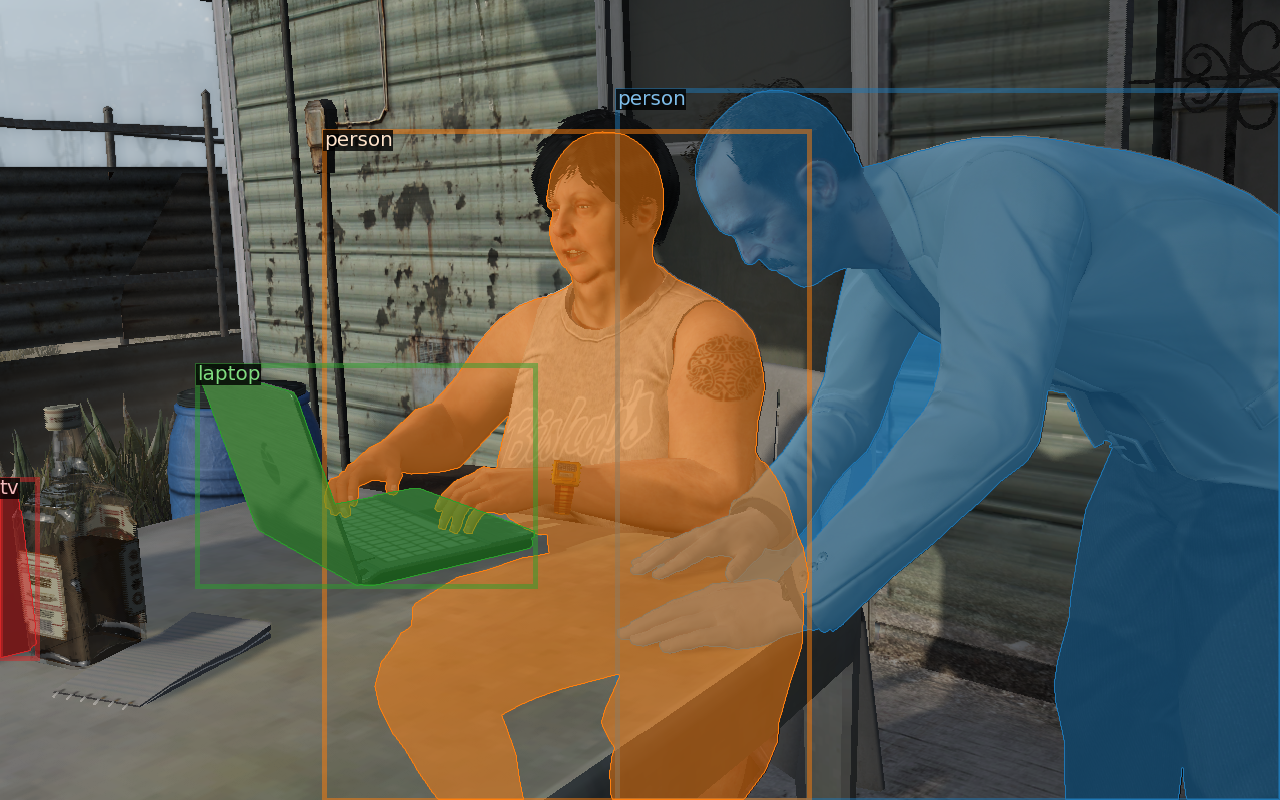
\includegraphics[align=c,width=0.23\linewidth]{fig/sailvos_results/21781_gt} &
    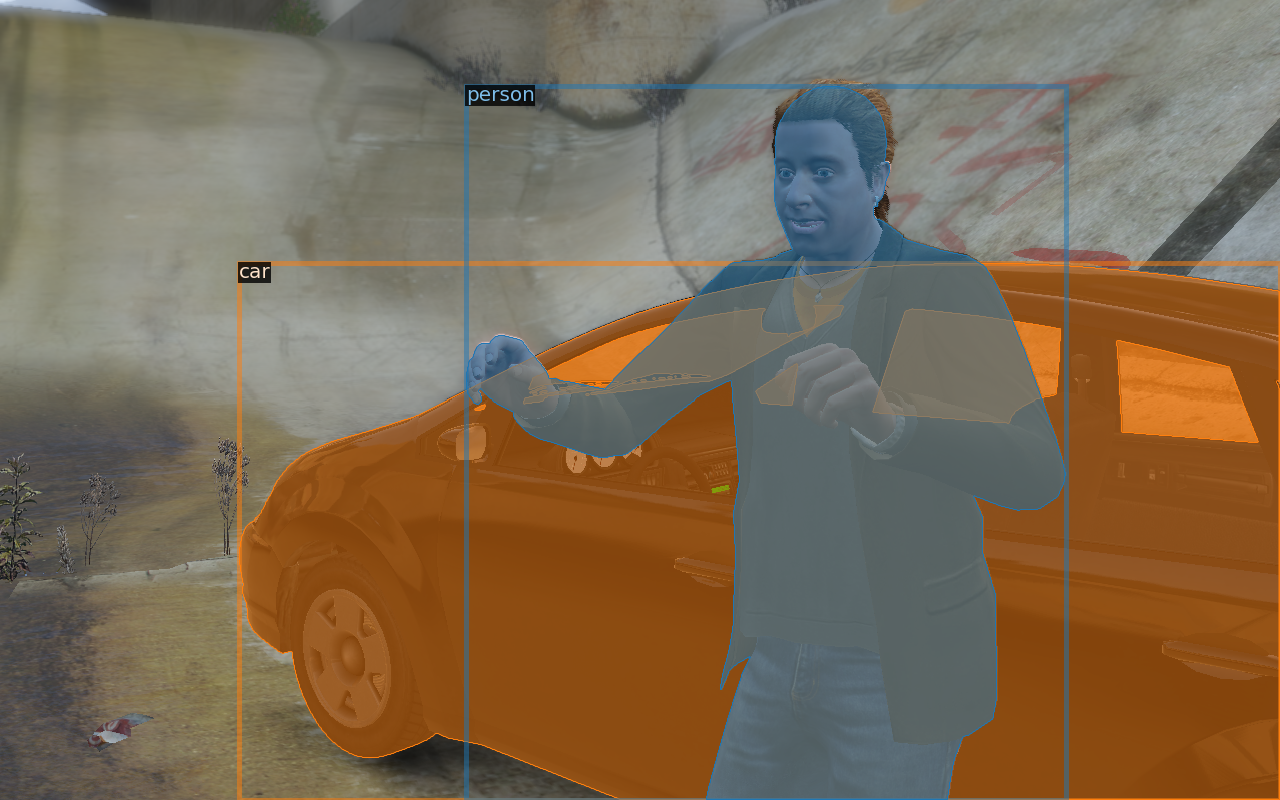
\includegraphics[align=c,width=0.23\linewidth]{fig/sailvos_results/10561_gt} &
    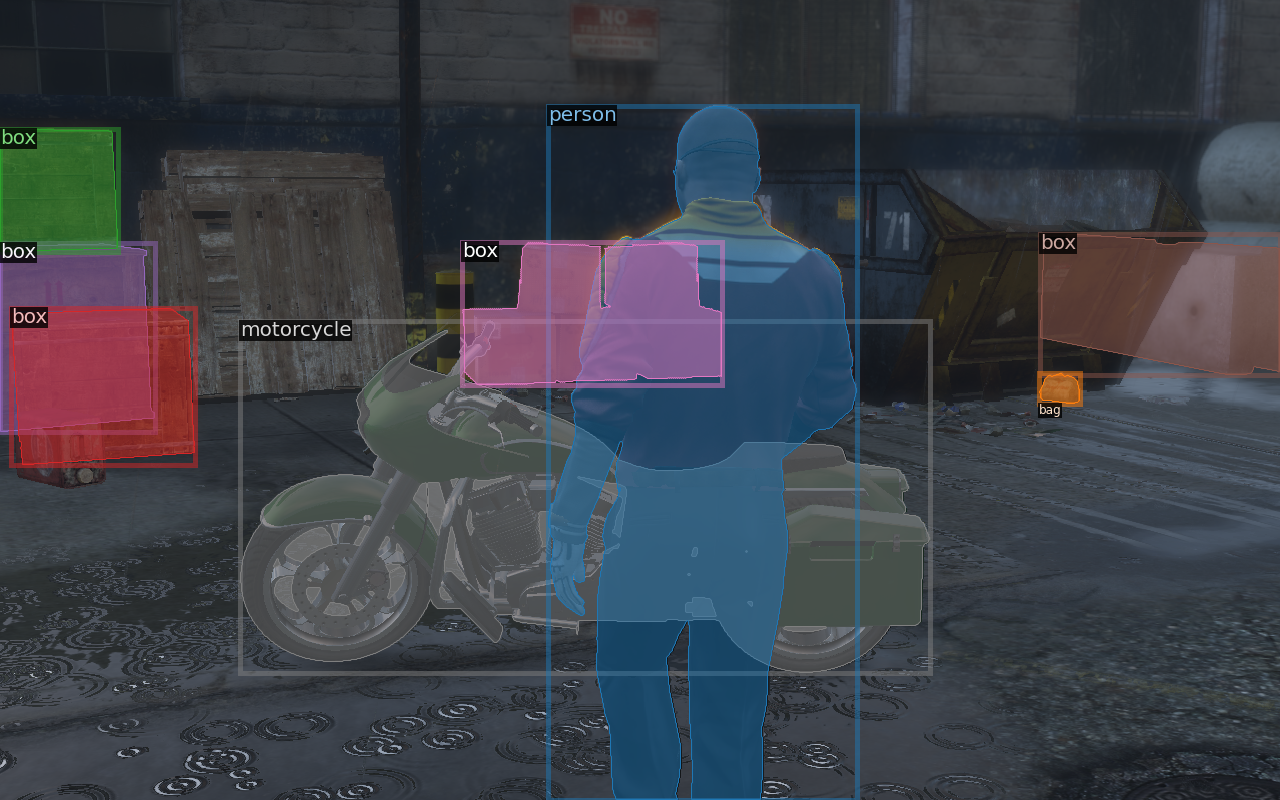
\includegraphics[align=c,width=0.23\linewidth]{fig/sailvos_results/14498_gt} &
    %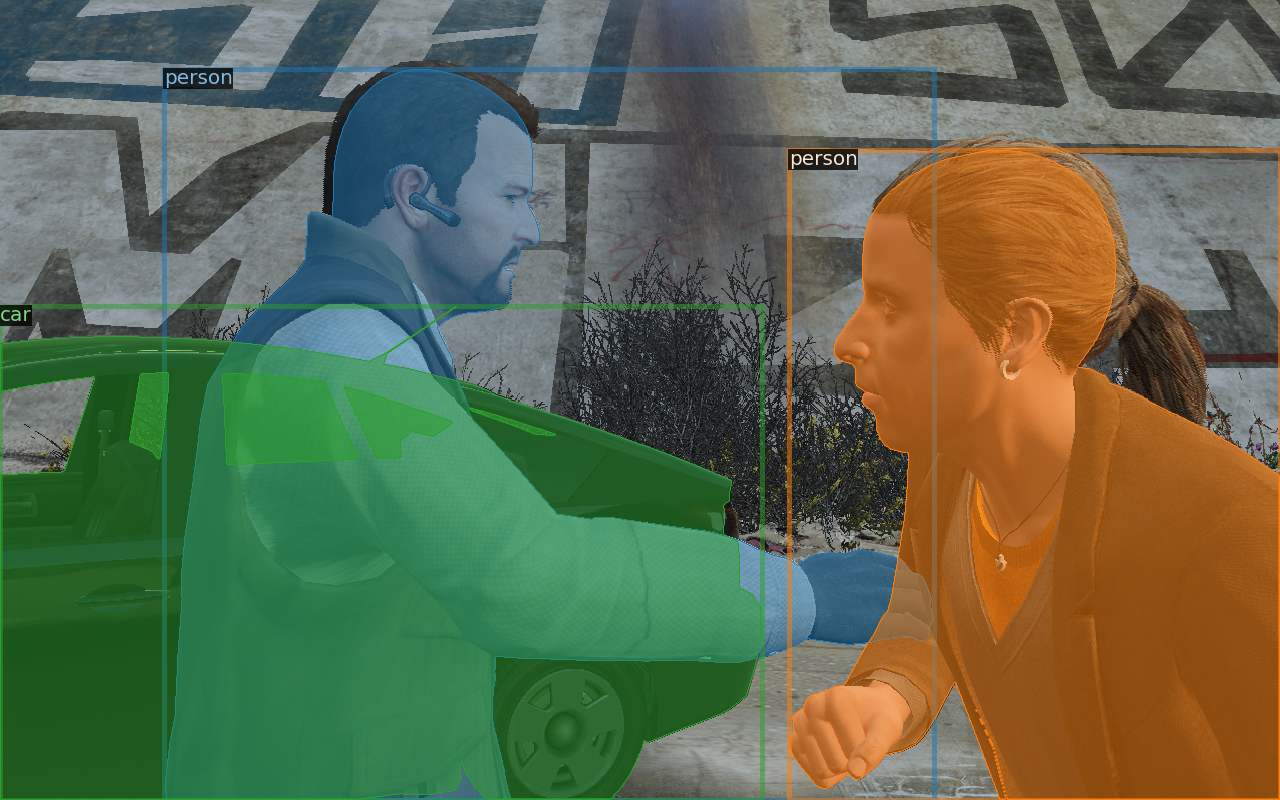
\includegraphics[align=c,width=0.23\linewidth]{fig/sailvos_results/11413_gt} &
    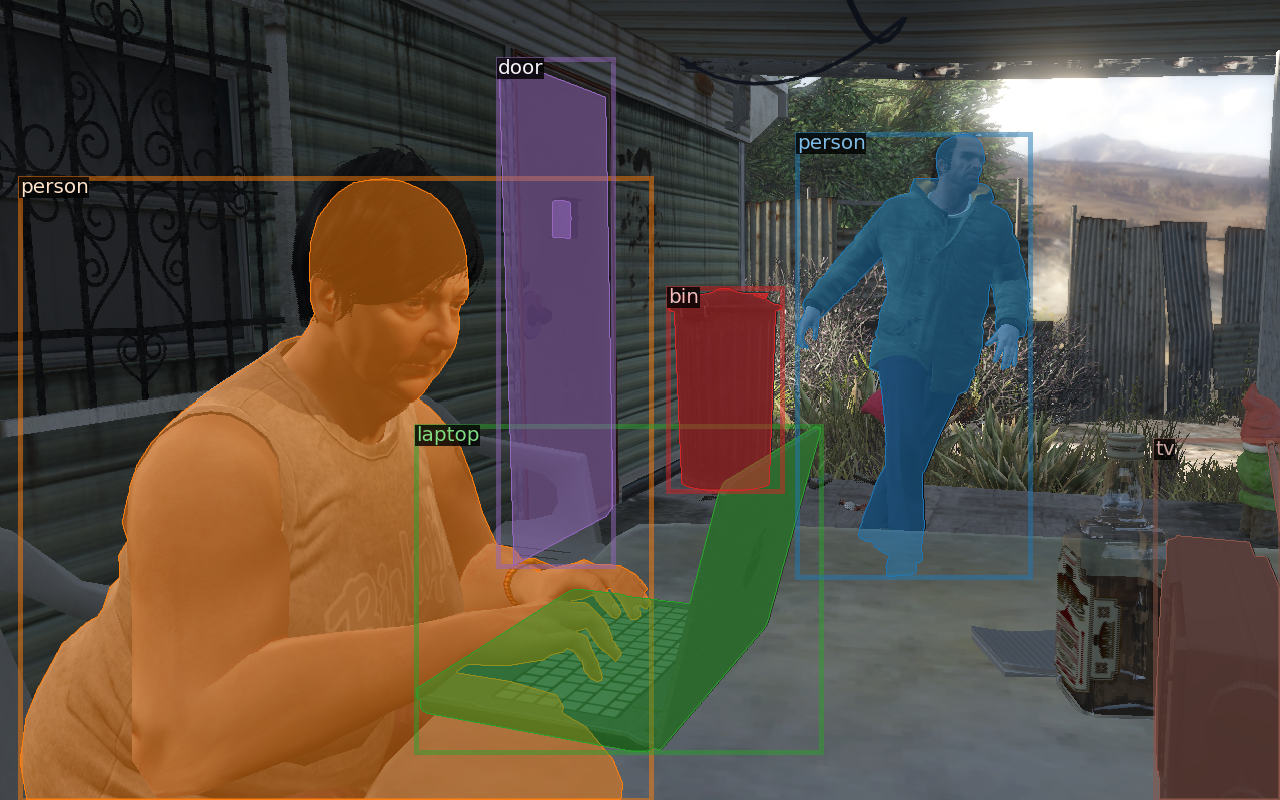
\includegraphics[align=c,width=0.23\linewidth]{fig/sailvos_results/22243_gt}
    \\
    % Baseline 
    \cite{hu2019sail} & 
    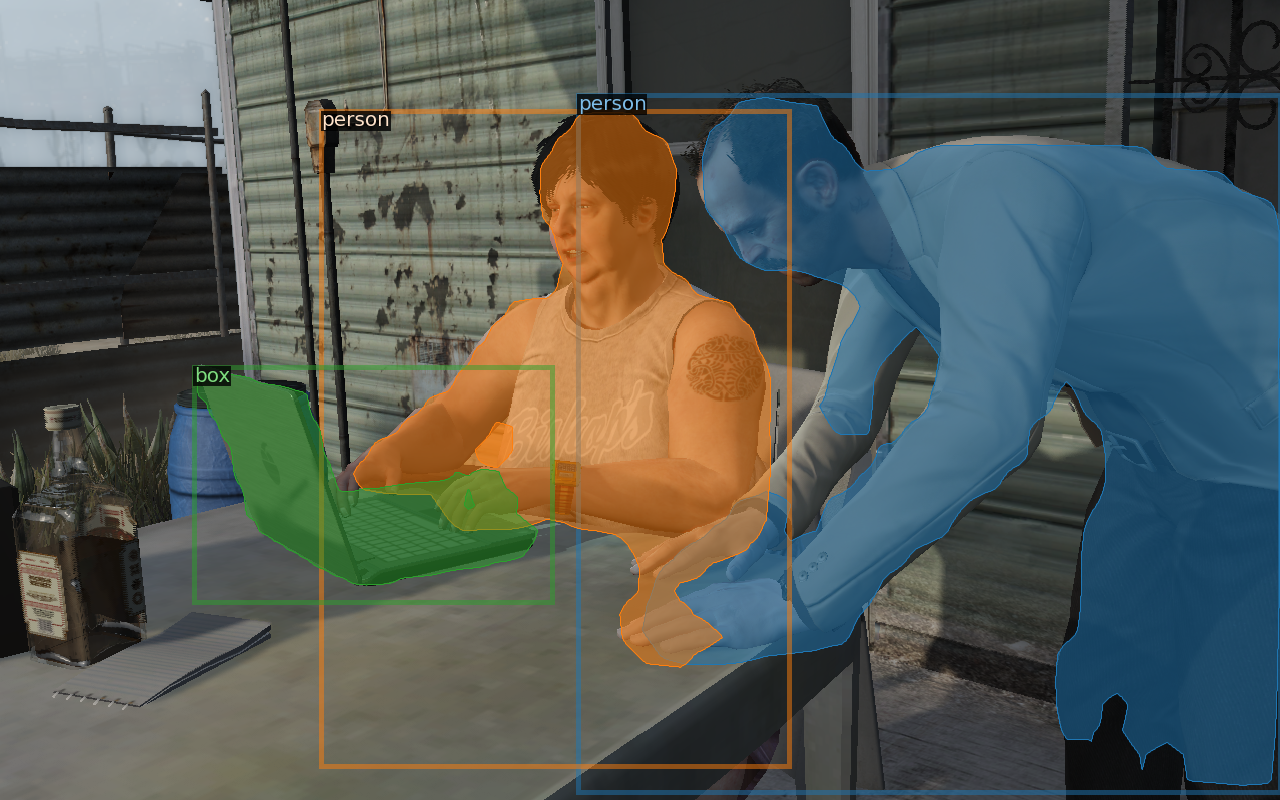
\includegraphics[align=c,width=0.23\linewidth]{fig/sailvos_results/21781_base} &
    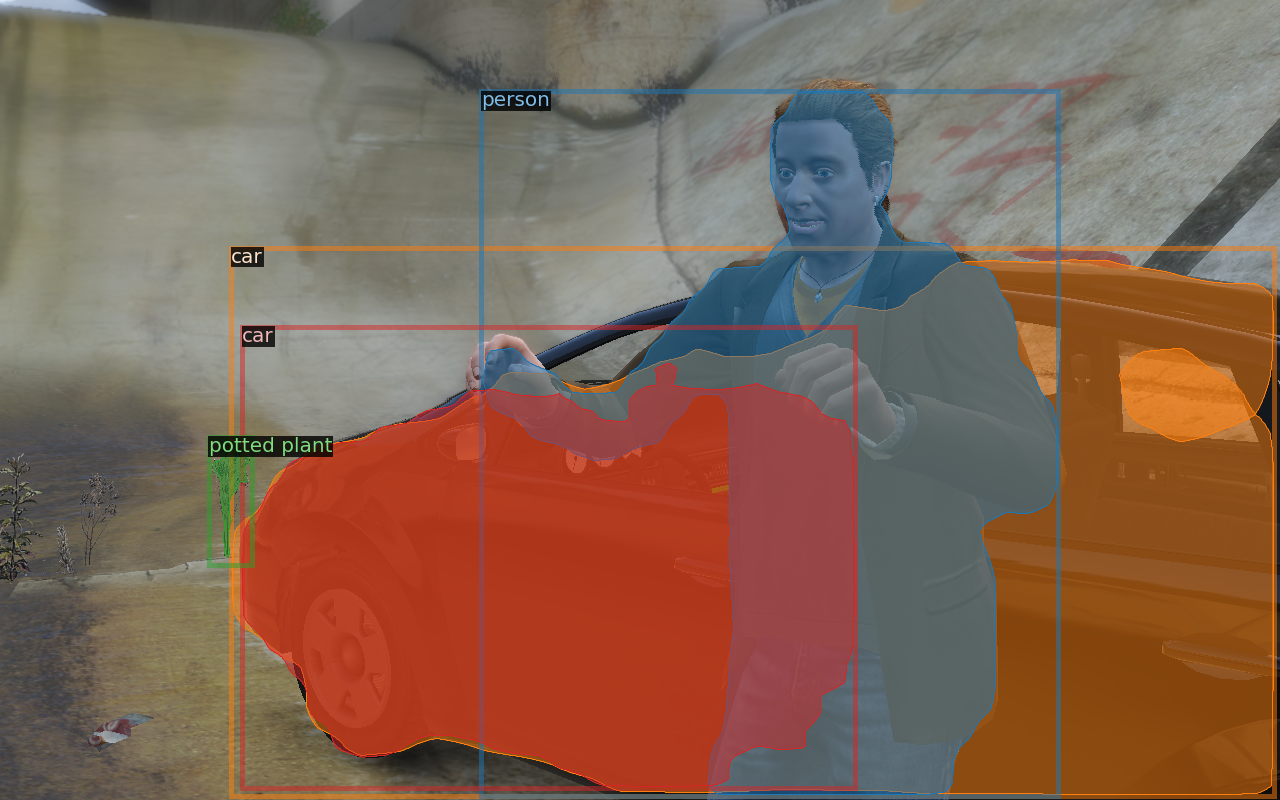
\includegraphics[align=c,width=0.23\linewidth]{fig/sailvos_results/10561_base} &
    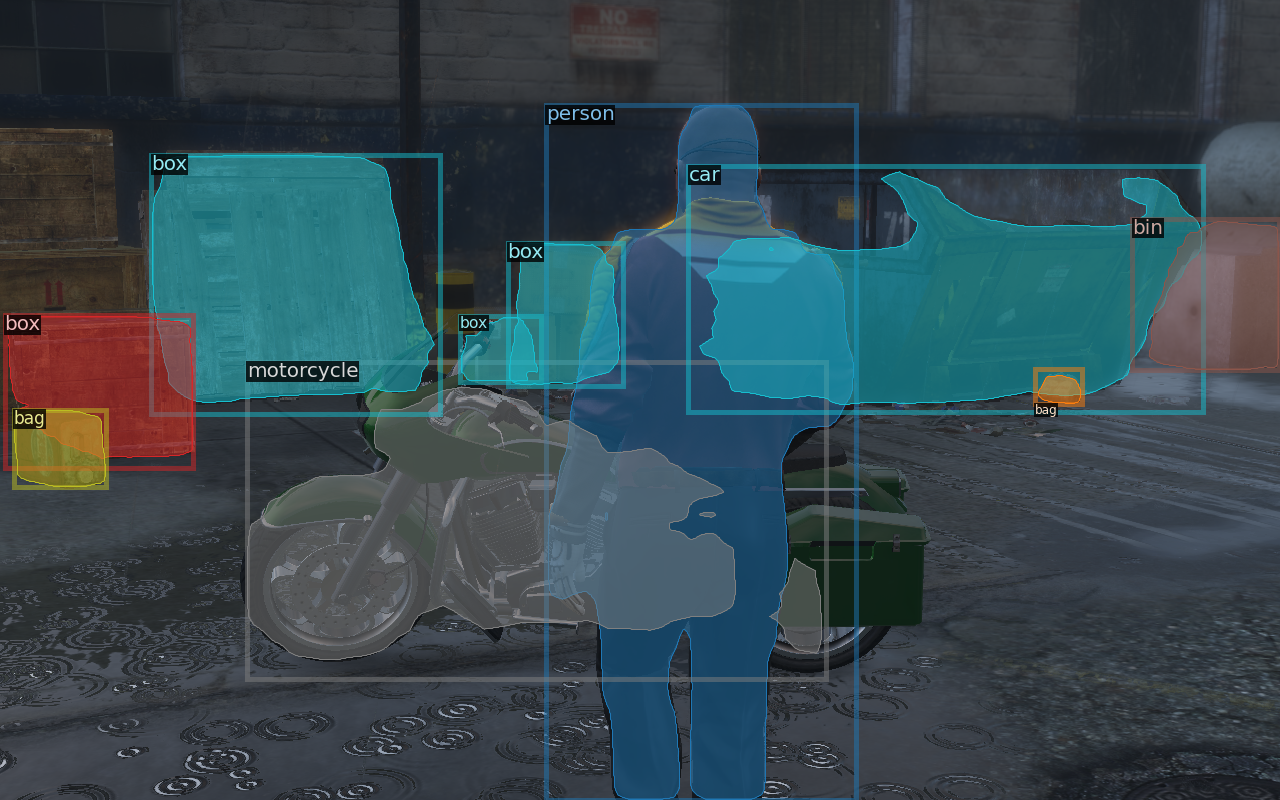
\includegraphics[align=c,width=0.23\linewidth]{fig/sailvos_results/14498_base} &
    %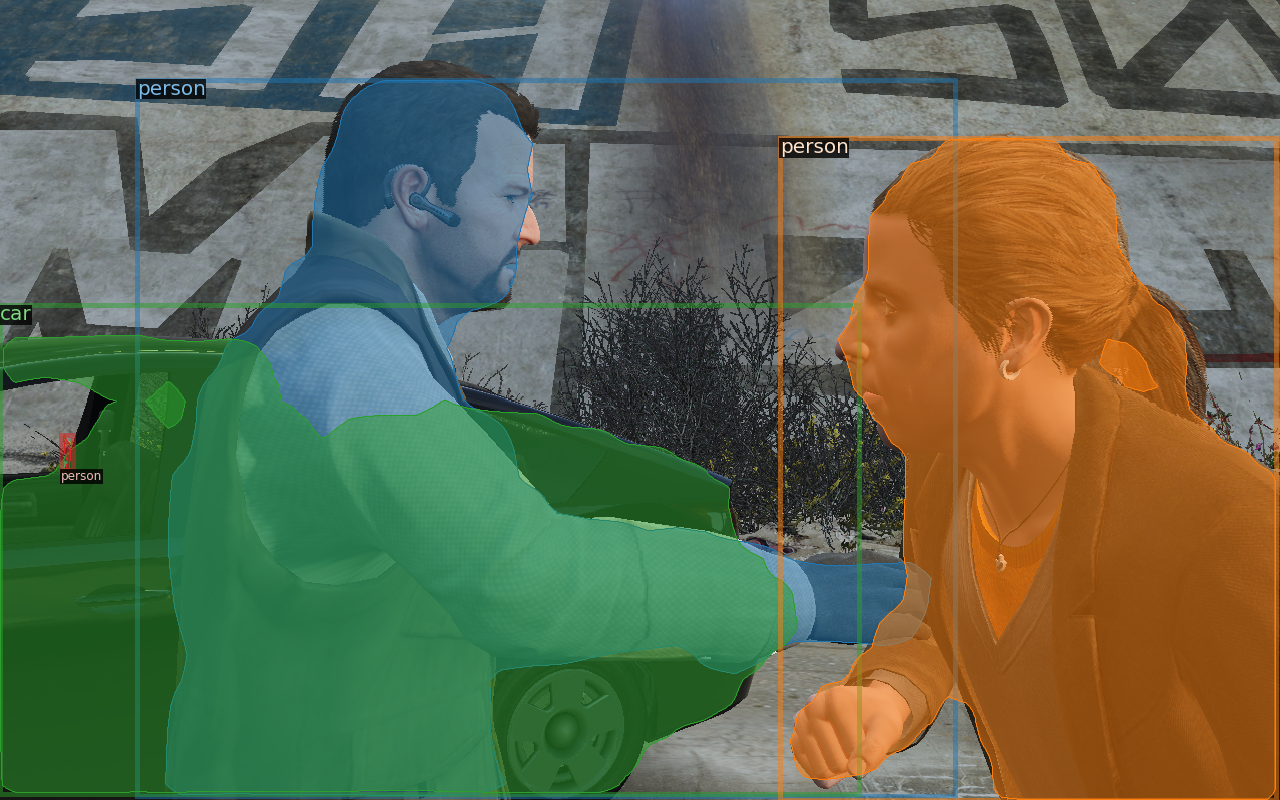
\includegraphics[align=c,width=0.23\linewidth]{fig/sailvos_results/11413_base} &
    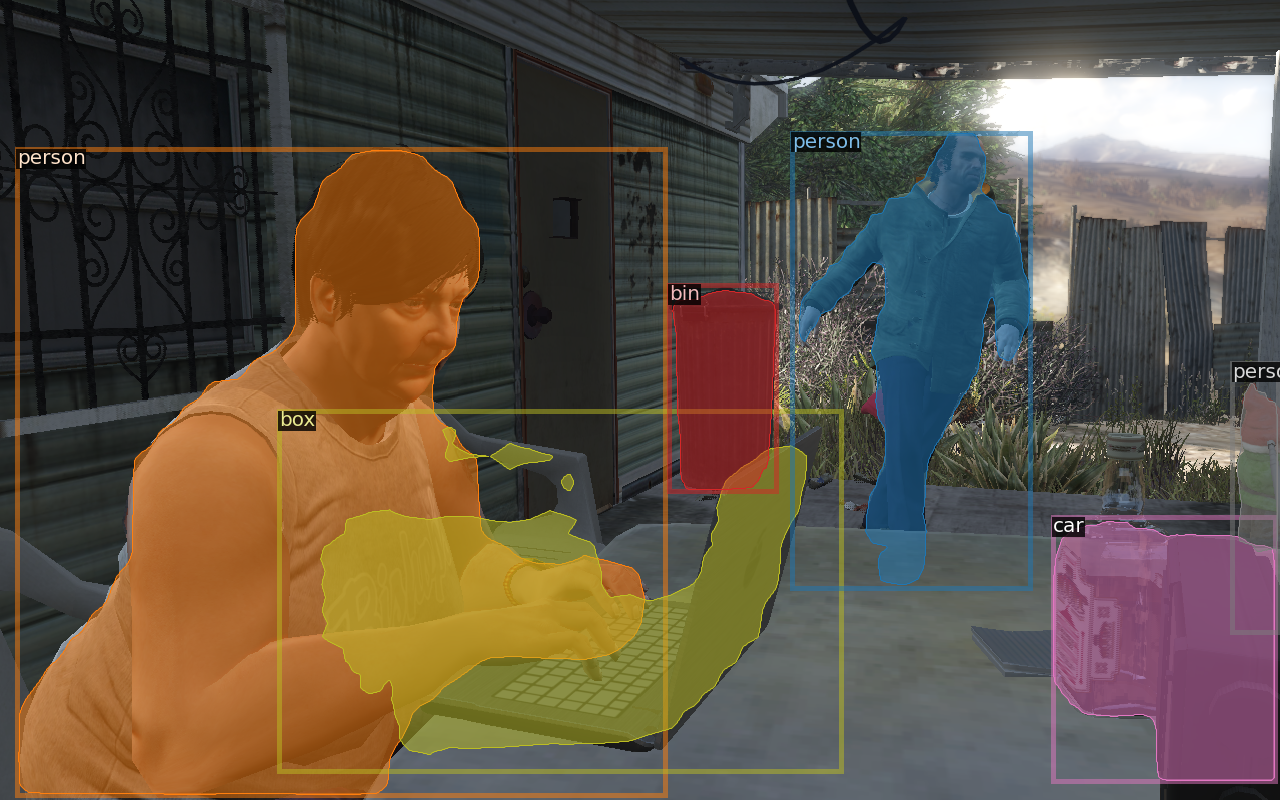
\includegraphics[align=c,width=0.23\linewidth]{fig/sailvos_results/22243_base}
    \\
    % Ours
    Ours &
    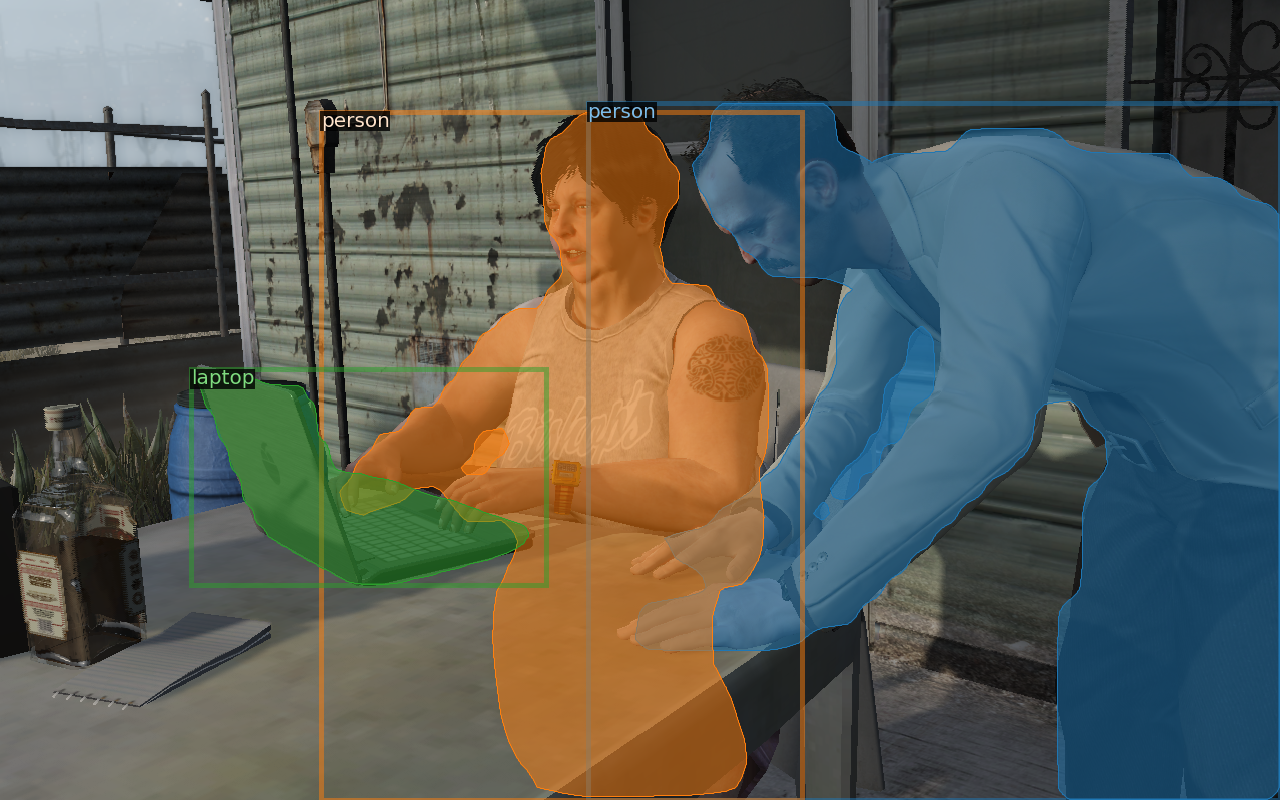
\includegraphics[align=c,width=0.23\linewidth]{fig/sailvos_results/21781_ours} &
    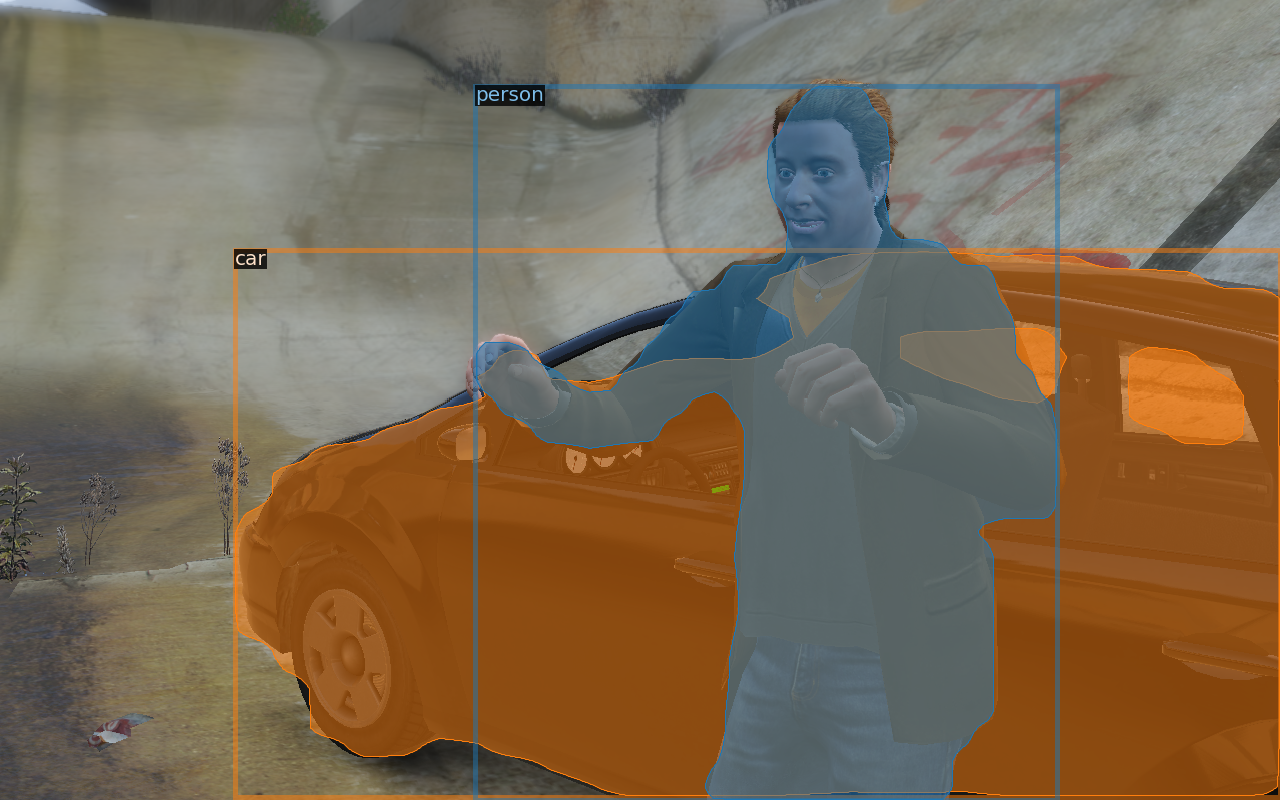
\includegraphics[align=c,width=0.23\linewidth]{fig/sailvos_results/10561_ours} &
    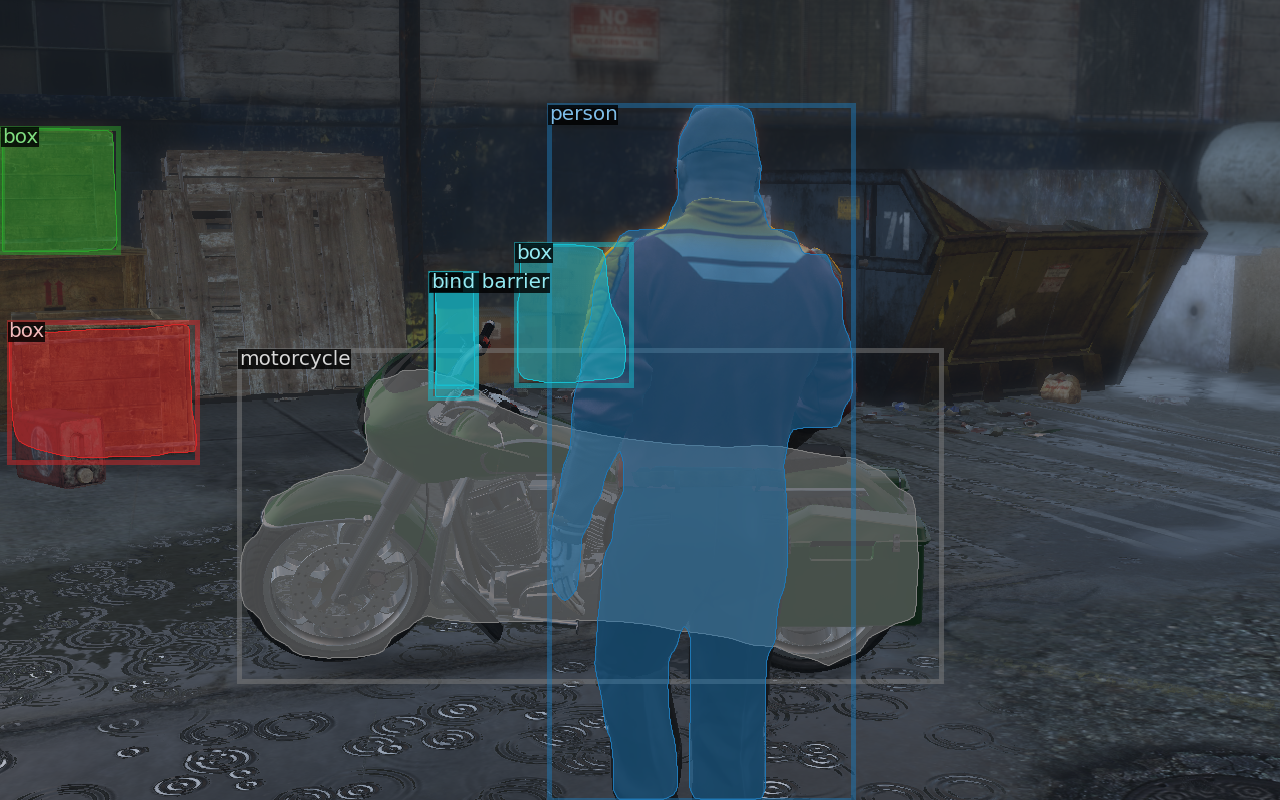
\includegraphics[align=c,width=0.23\linewidth]{fig/sailvos_results/14498_ours} &
    %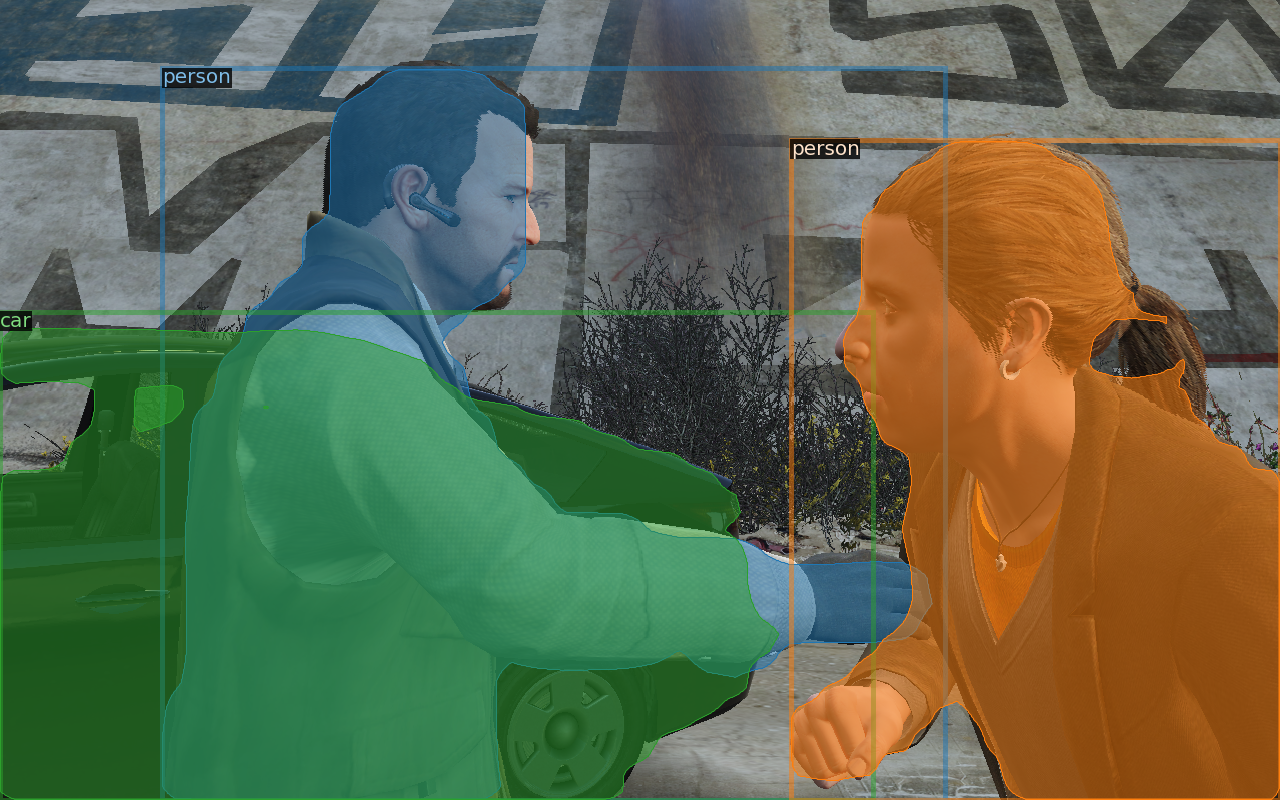
\includegraphics[align=c,width=0.23\linewidth]{fig/sailvos_results/11413_ours} &
    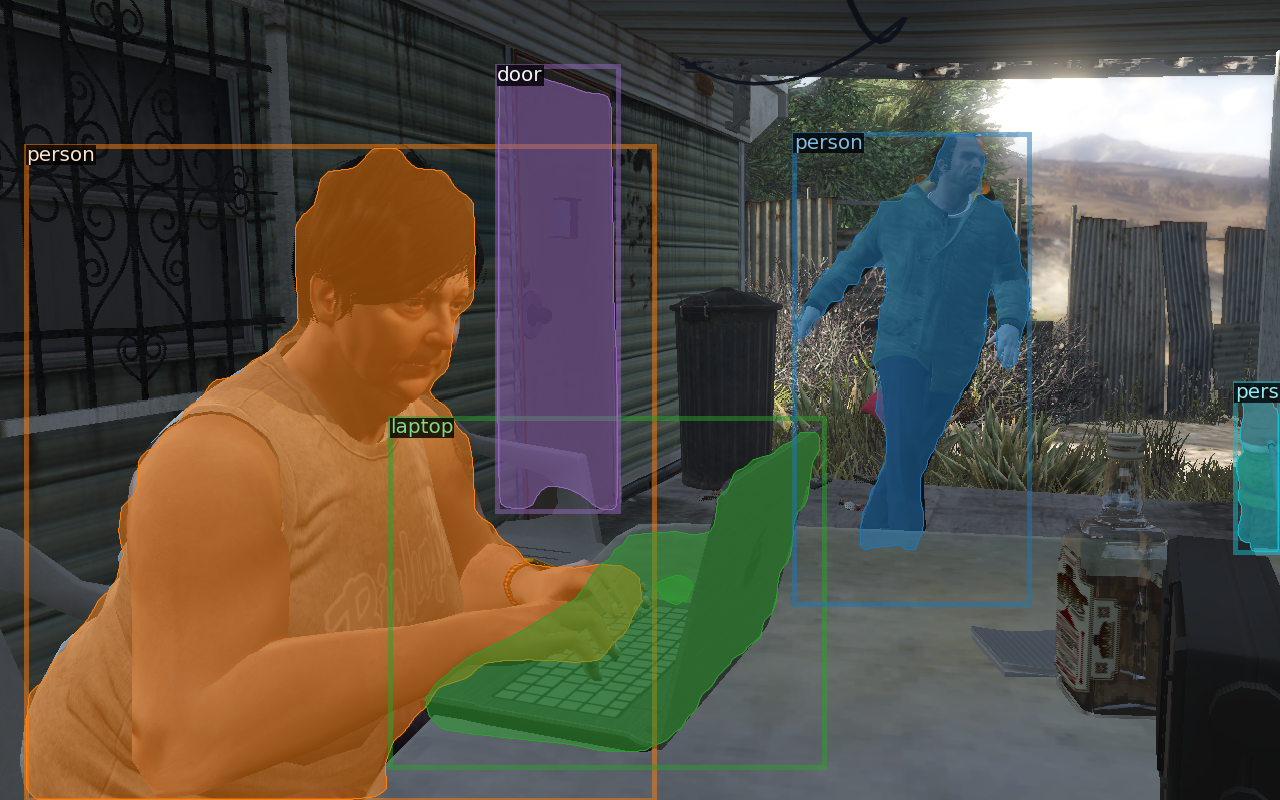
\includegraphics[align=c,width=0.23\linewidth]{fig/sailvos_results/22243_ours}
    \end{tabular}
    \vspace{-0.25cm}
    \caption{Qualitative comparison with~\cite{hu2019sail} on SAIL-VOS dataset in the class-specific setting.
    %\as{using the class-specific setting?}.
    }
    \label{fig:qual_result}
    \vspace{-0.25cm}
    \end{figure*}
    
    
    
    %\begin{tabular}{ccccc}
    %% GT
    %GT & 
    %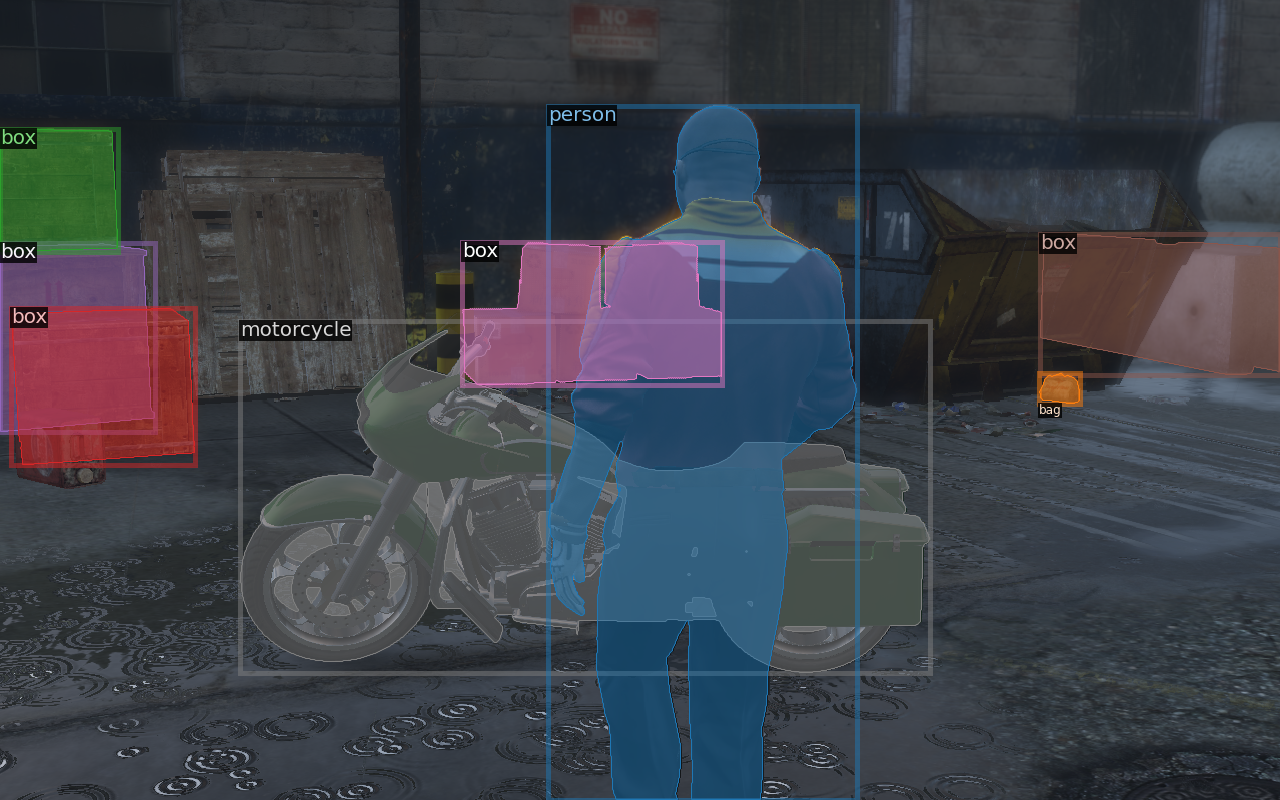
\includegraphics[align=c,width=0.23\linewidth]{fig/sailvos_results/14498_gt} &
    %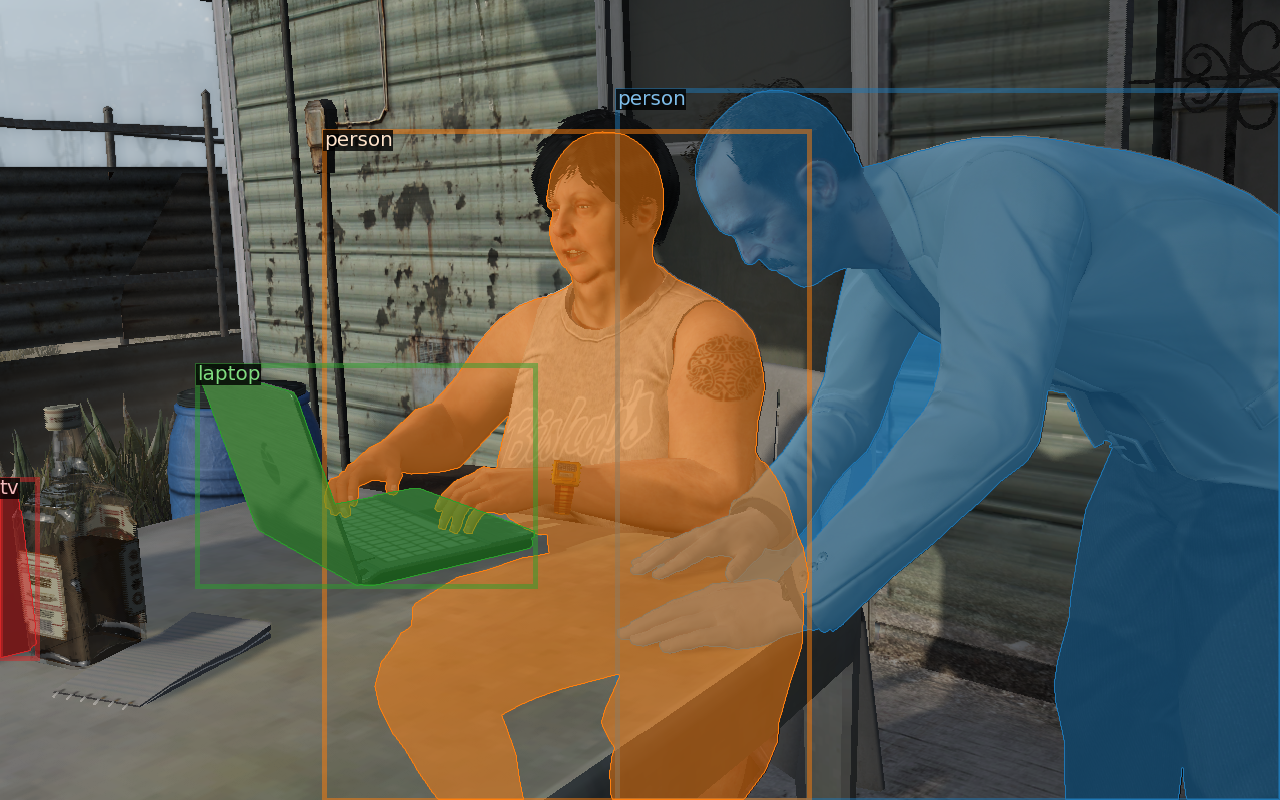
\includegraphics[align=c,width=0.23\linewidth]{fig/sailvos_results/21781_gt} &
    %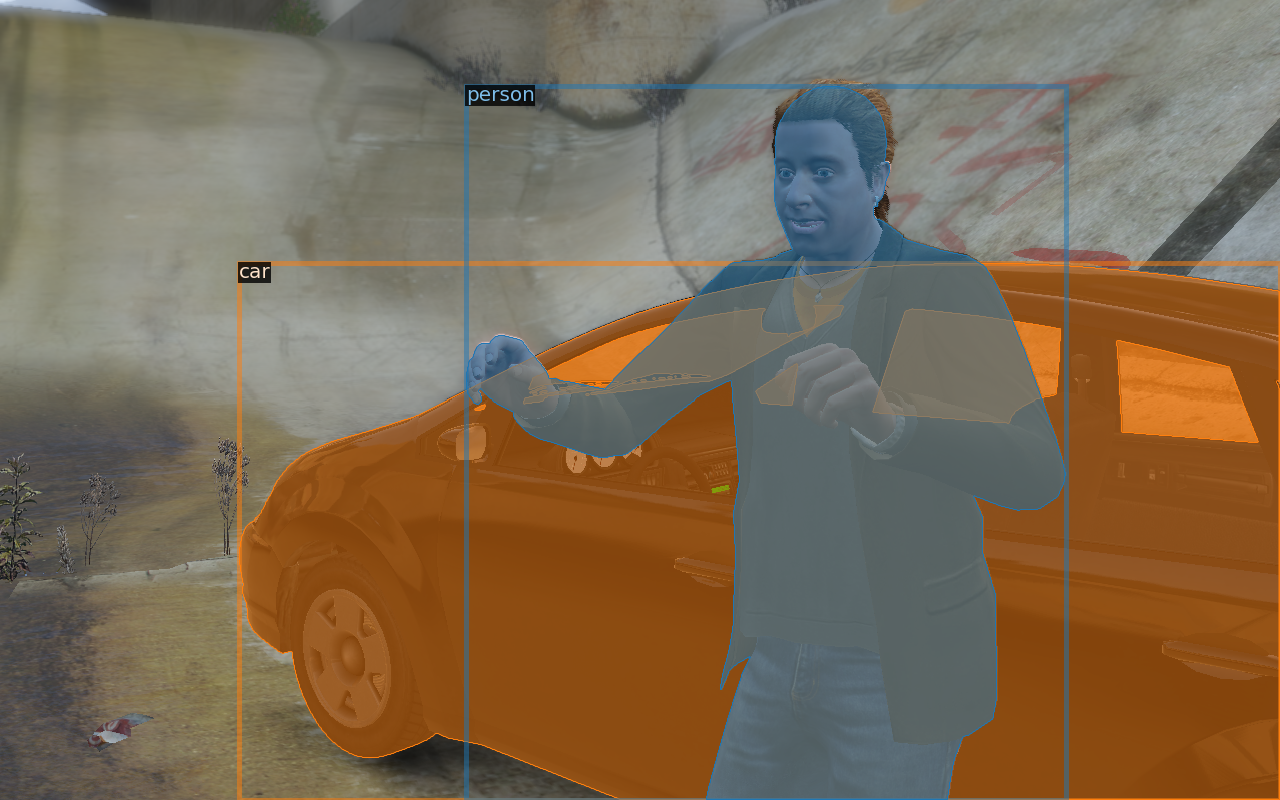
\includegraphics[align=c,width=0.23\linewidth]{fig/sailvos_results/10561_gt} &
    %%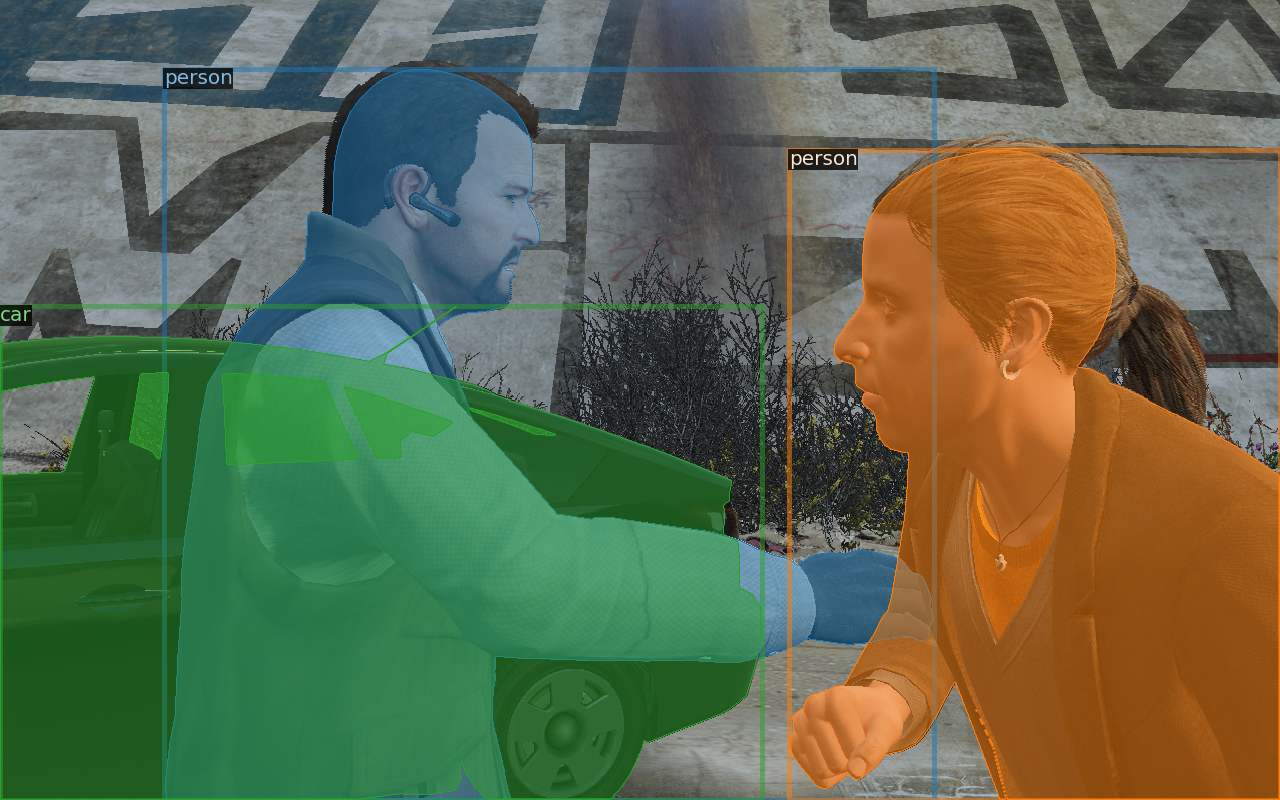
\includegraphics[align=c,width=0.23\linewidth]{fig/sailvos_results/11413_gt} &
    %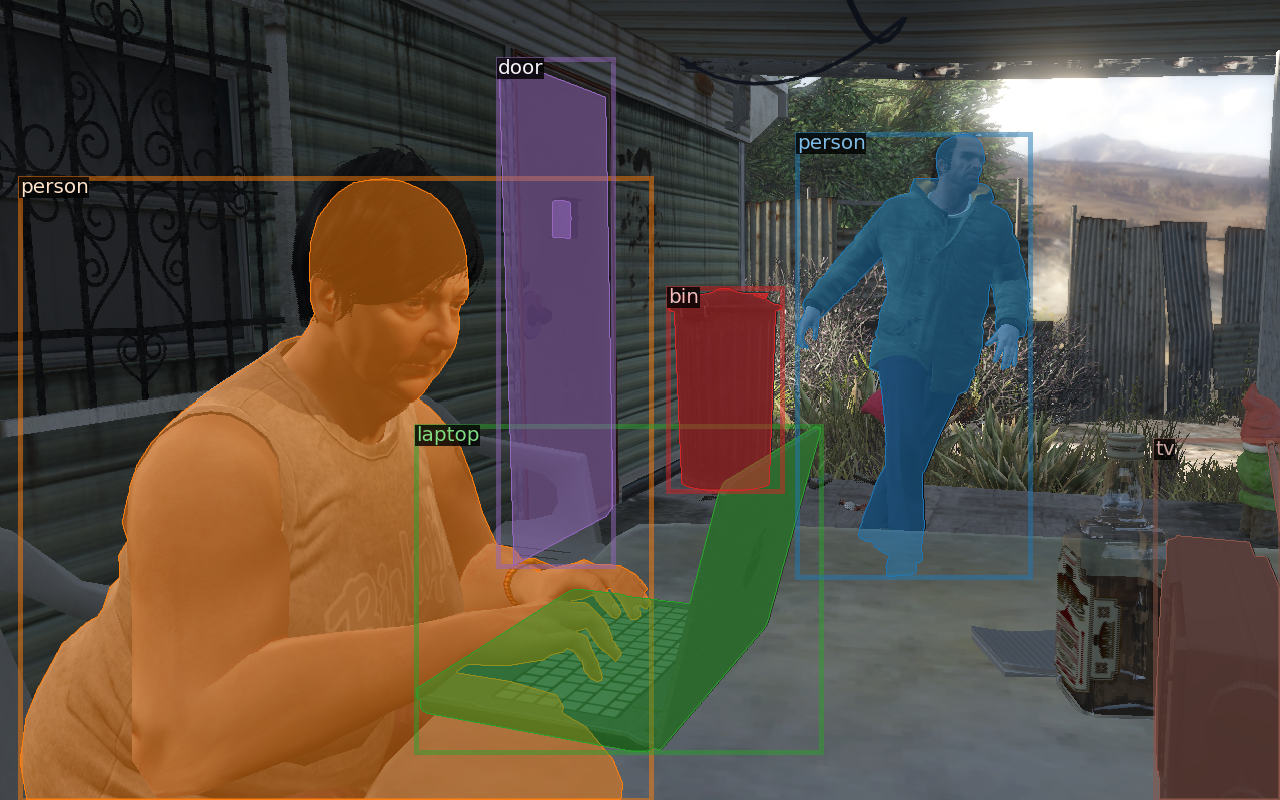
\includegraphics[align=c,width=0.23\linewidth]{fig/sailvos_results/22243_gt}
    %\\
    %% Baseline 
    %\cite{hu2019sail} & 
    %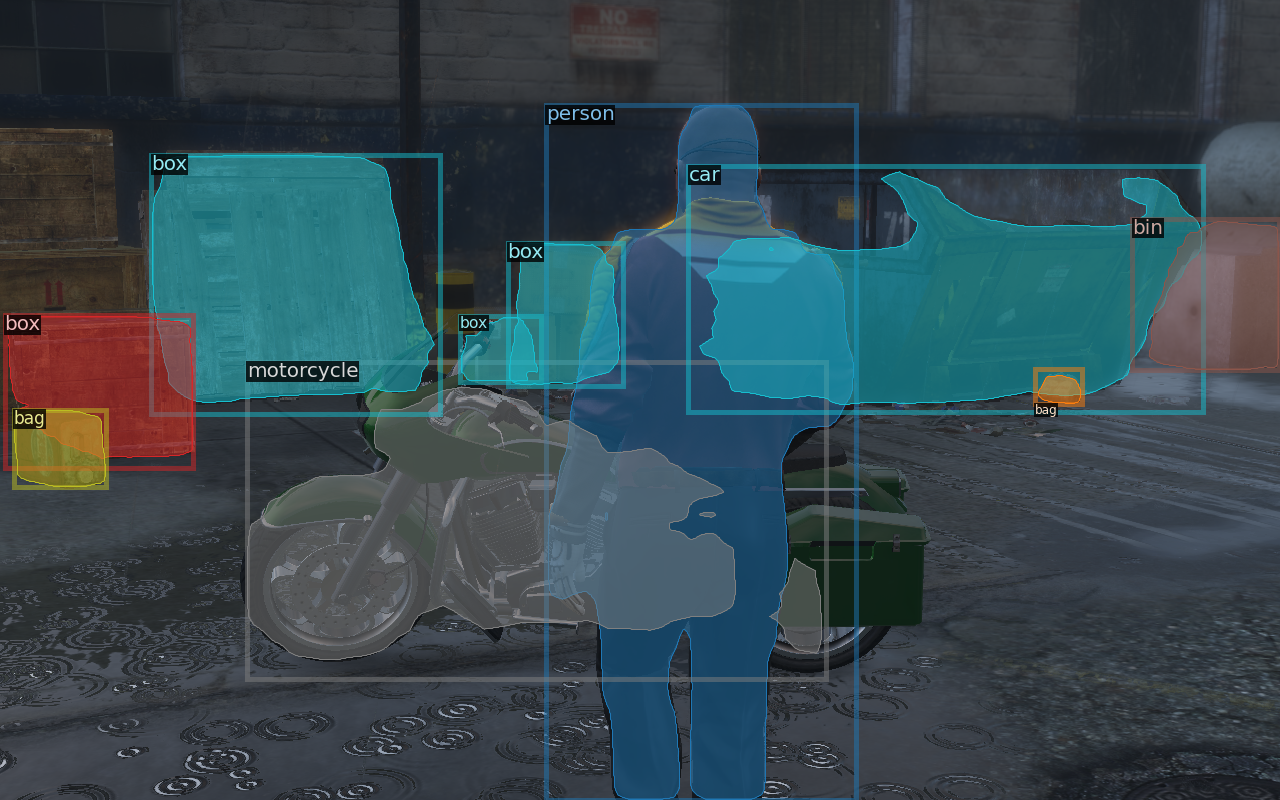
\includegraphics[align=c,width=0.23\linewidth]{fig/sailvos_results/14498_base} &
    %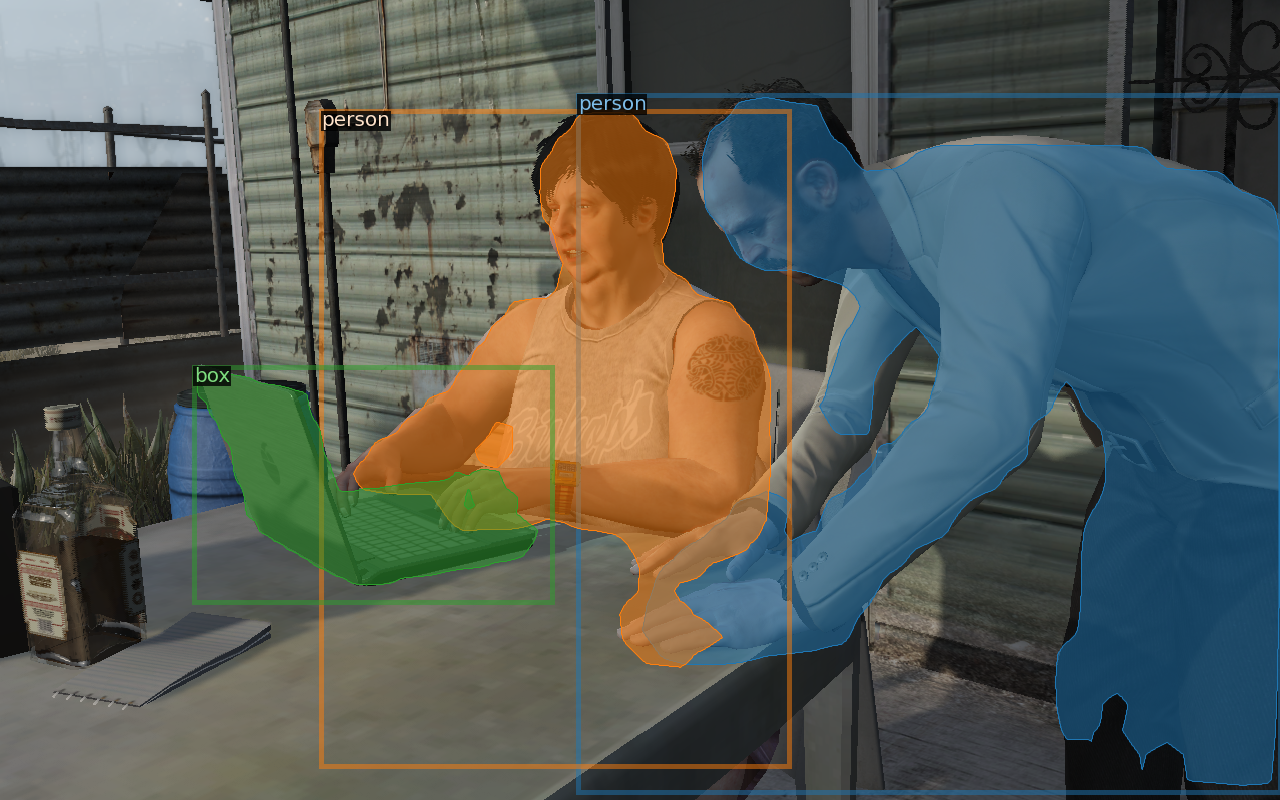
\includegraphics[align=c,width=0.23\linewidth]{fig/sailvos_results/21781_base} &
    %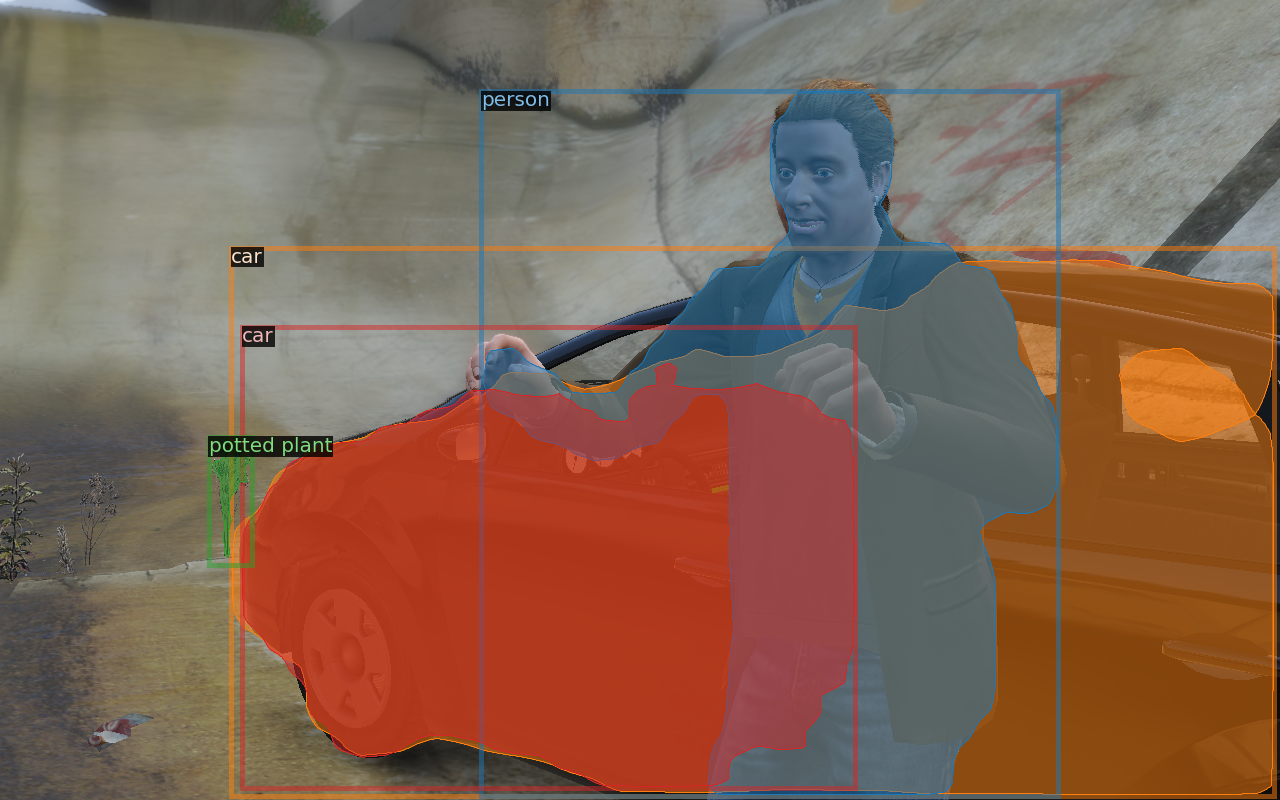
\includegraphics[align=c,width=0.23\linewidth]{fig/sailvos_results/10561_base} &
    %%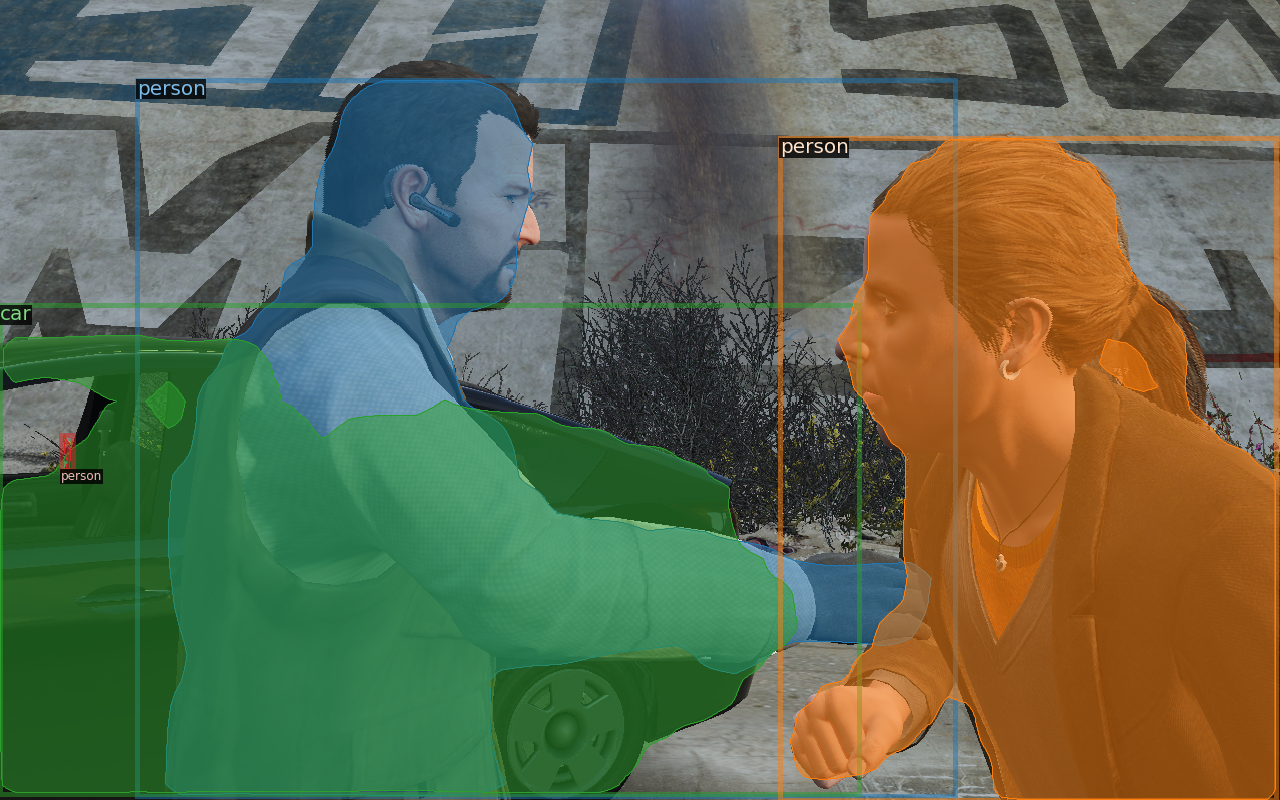
\includegraphics[align=c,width=0.23\linewidth]{fig/sailvos_results/11413_base} &
    %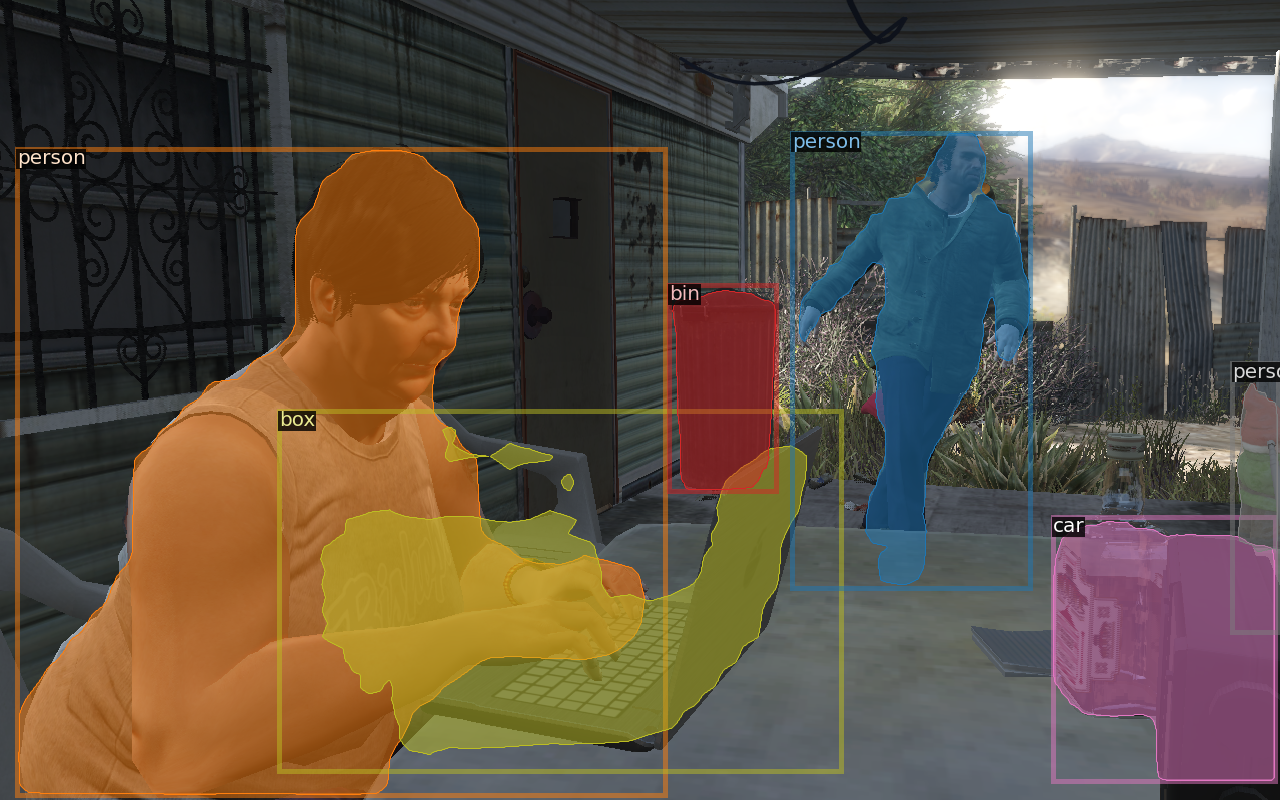
\includegraphics[align=c,width=0.23\linewidth]{fig/sailvos_results/22243_base}
    %\\
    %% Ours
    %Ours &
    %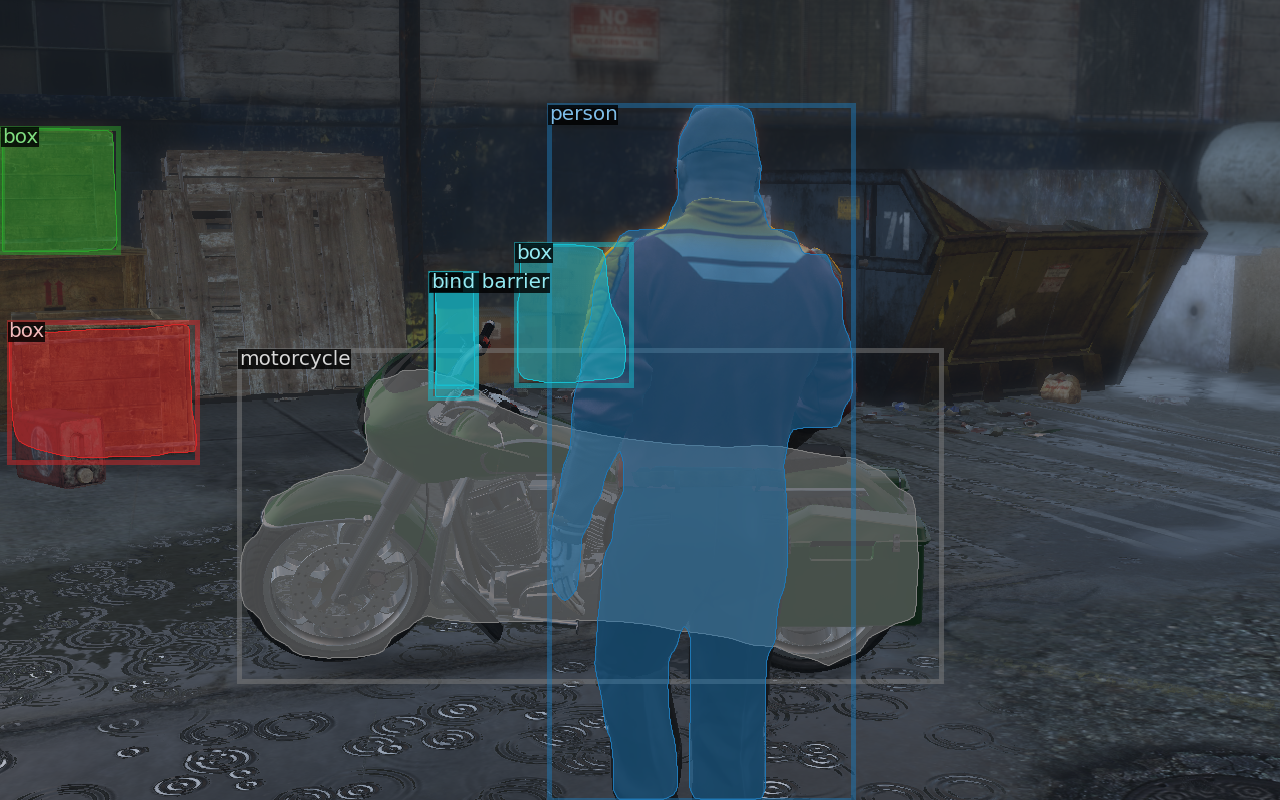
\includegraphics[align=c,width=0.23\linewidth]{fig/sailvos_results/14498_ours} &
    %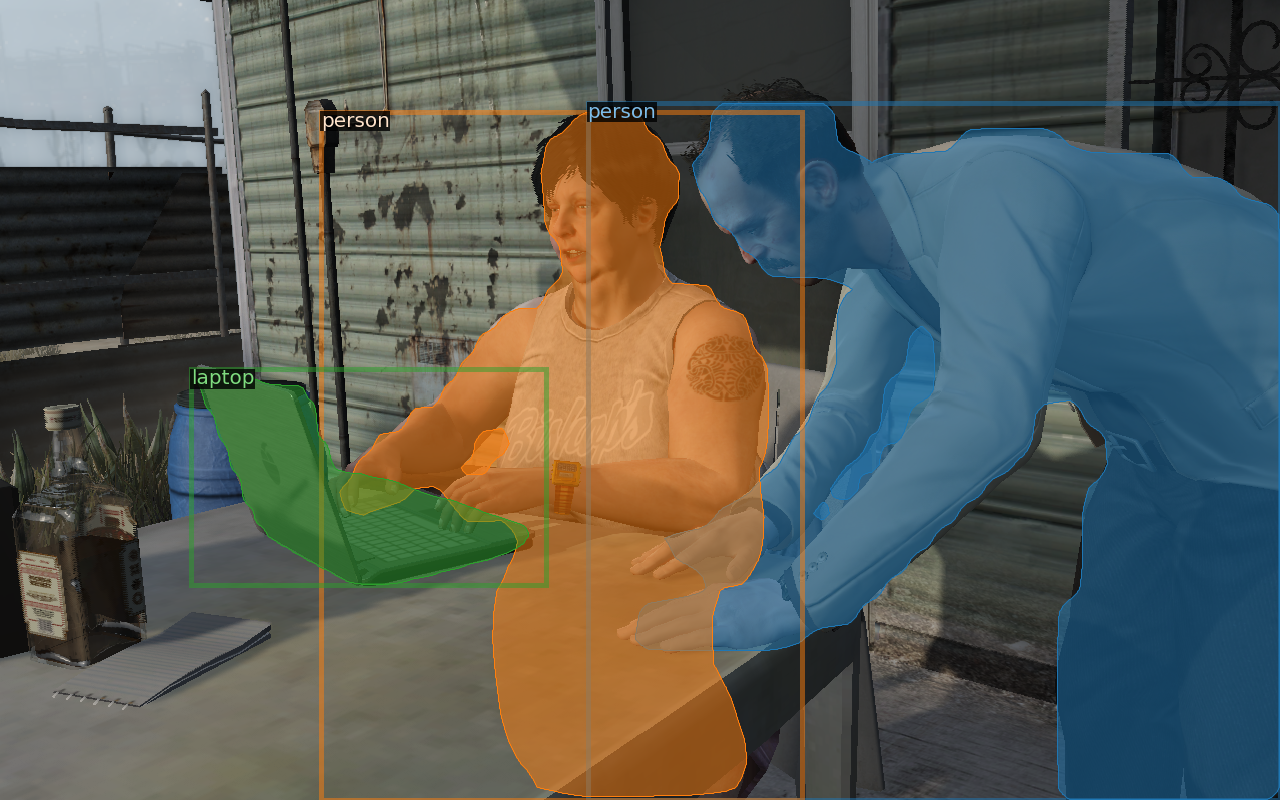
\includegraphics[align=c,width=0.23\linewidth]{fig/sailvos_results/21781_ours} &
    %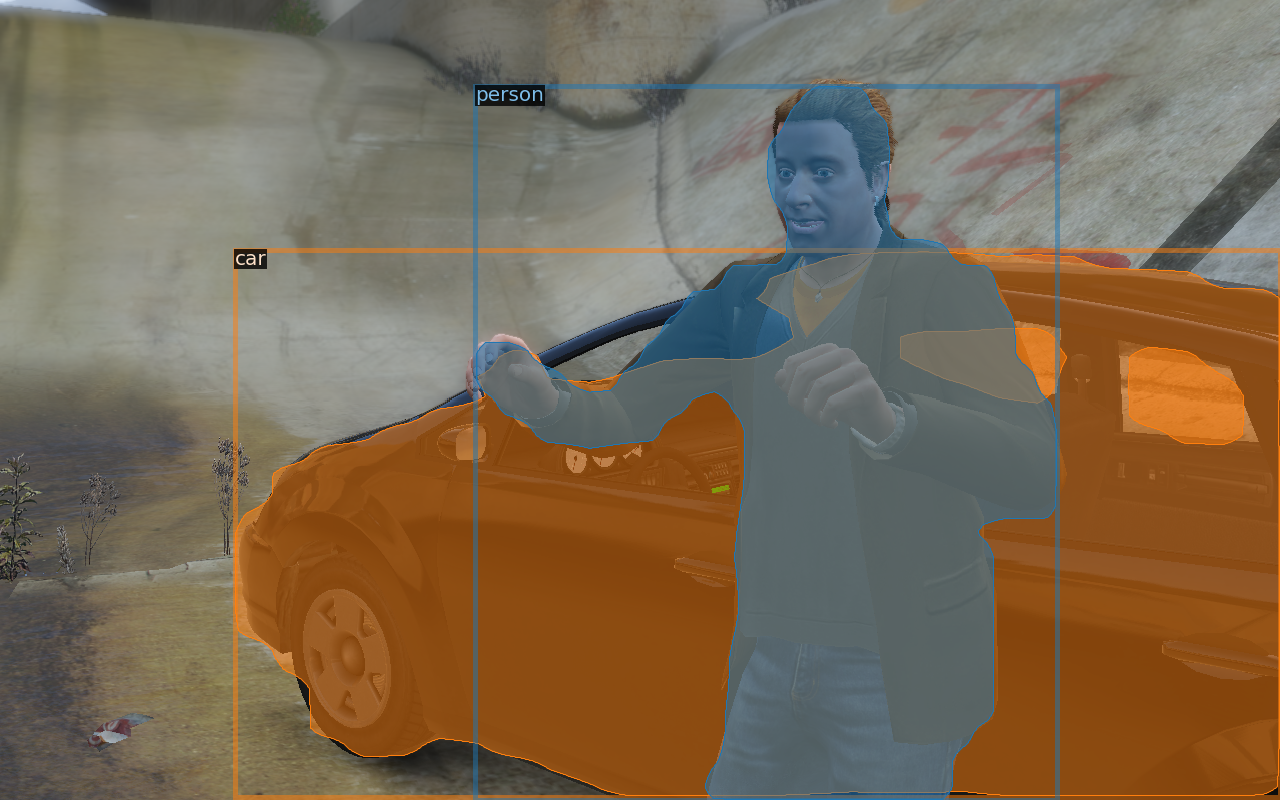
\includegraphics[align=c,width=0.23\linewidth]{fig/sailvos_results/10561_ours} &
    %%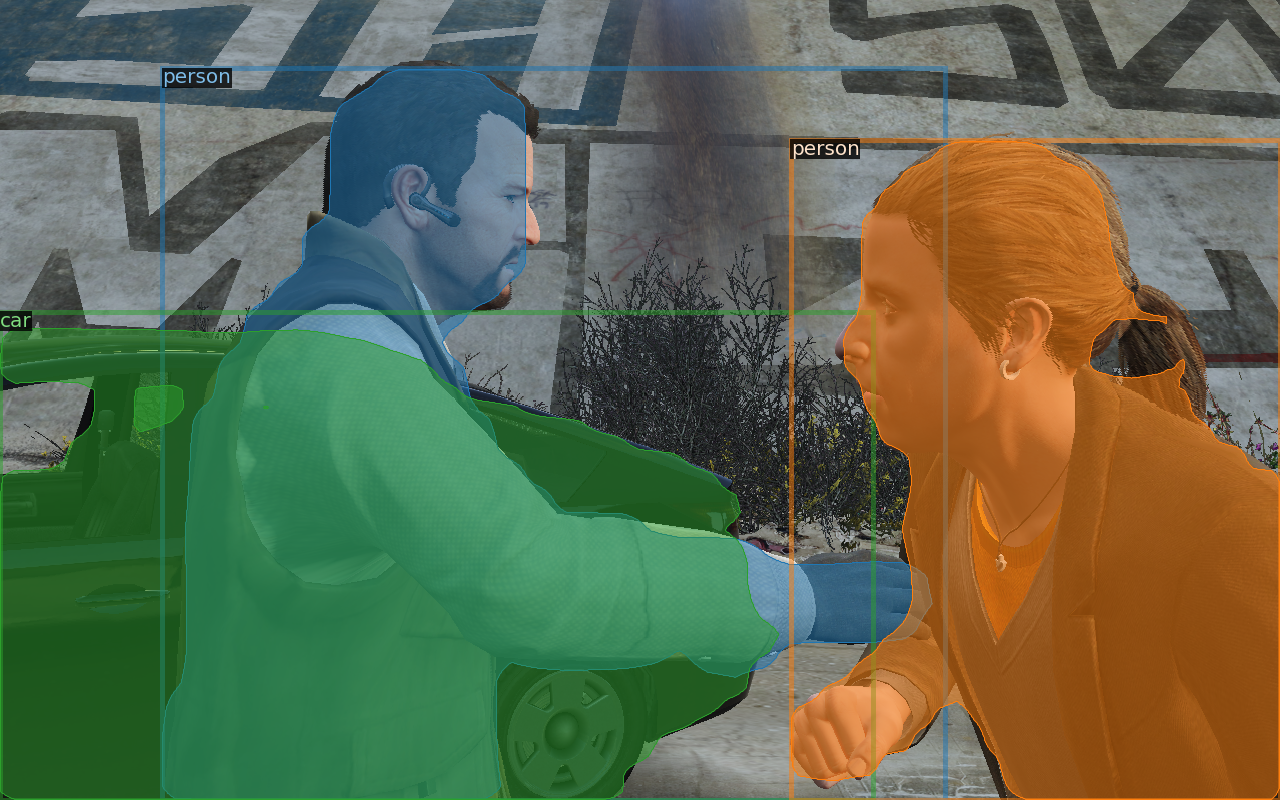
\includegraphics[align=c,width=0.23\linewidth]{fig/sailvos_results/11413_ours} &
    %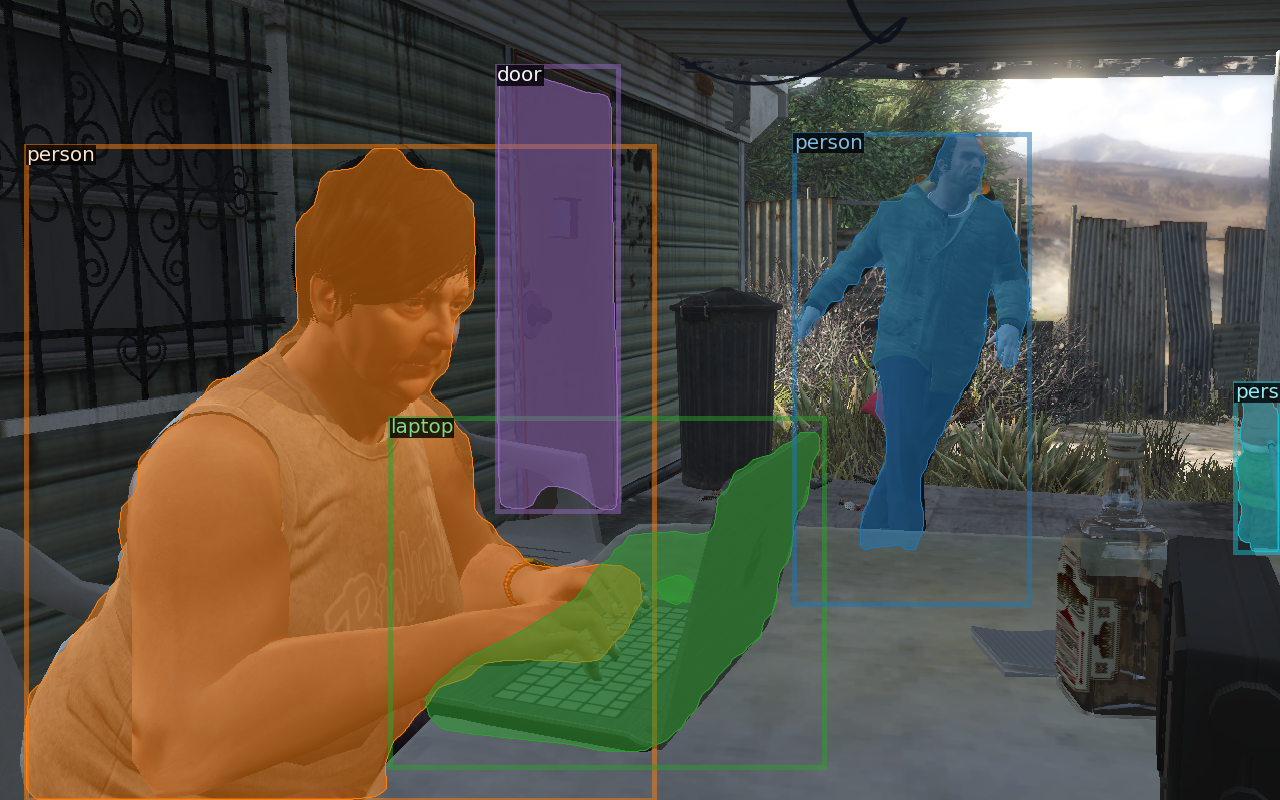
\includegraphics[align=c,width=0.23\linewidth]{fig/sailvos_results/22243_ours}
    %\end{tabular}
    
    %\begin{tabular}{ccc}
    %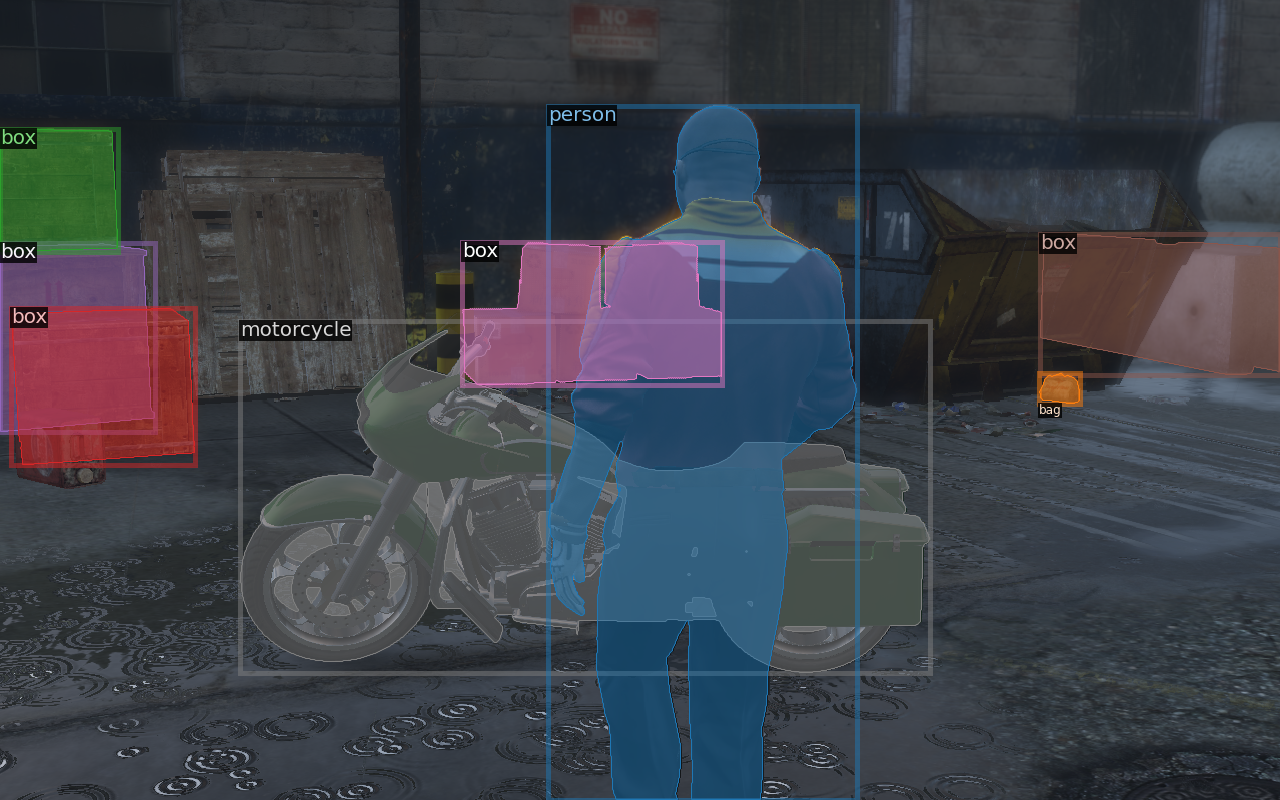
\includegraphics[width=0.31\linewidth]{fig/sailvos_results/14498_gt} & 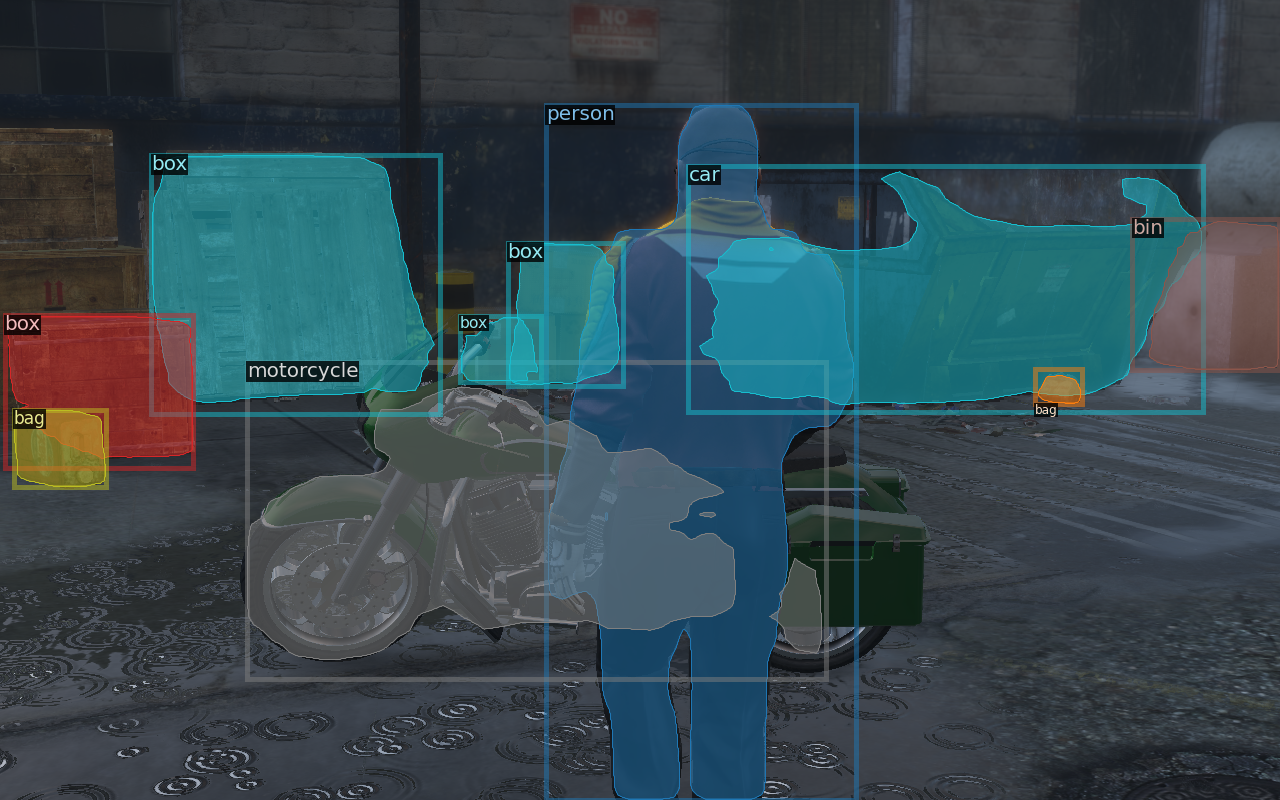
\includegraphics[width=0.31\linewidth]{fig/sailvos_results/14498_base} & 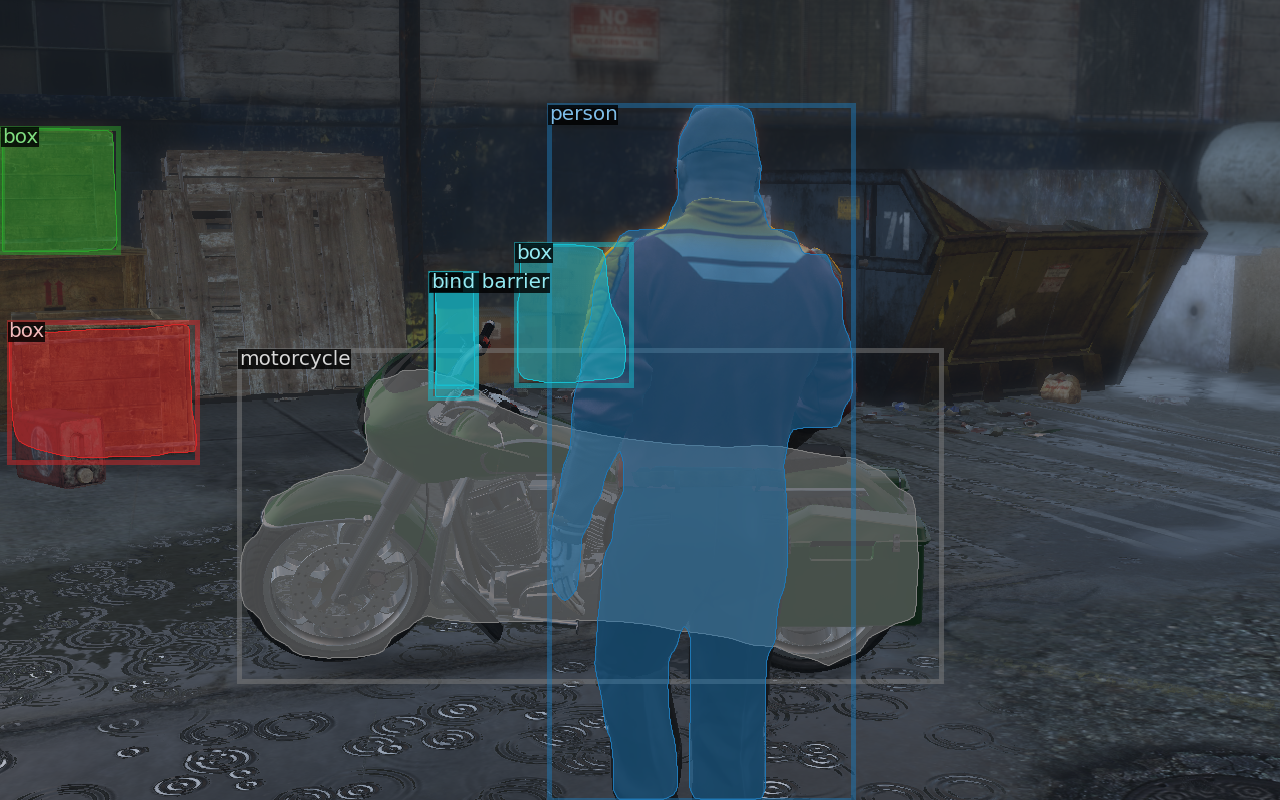
\includegraphics[width=0.31\linewidth]{fig/sailvos_results/14498_ours}\\
    %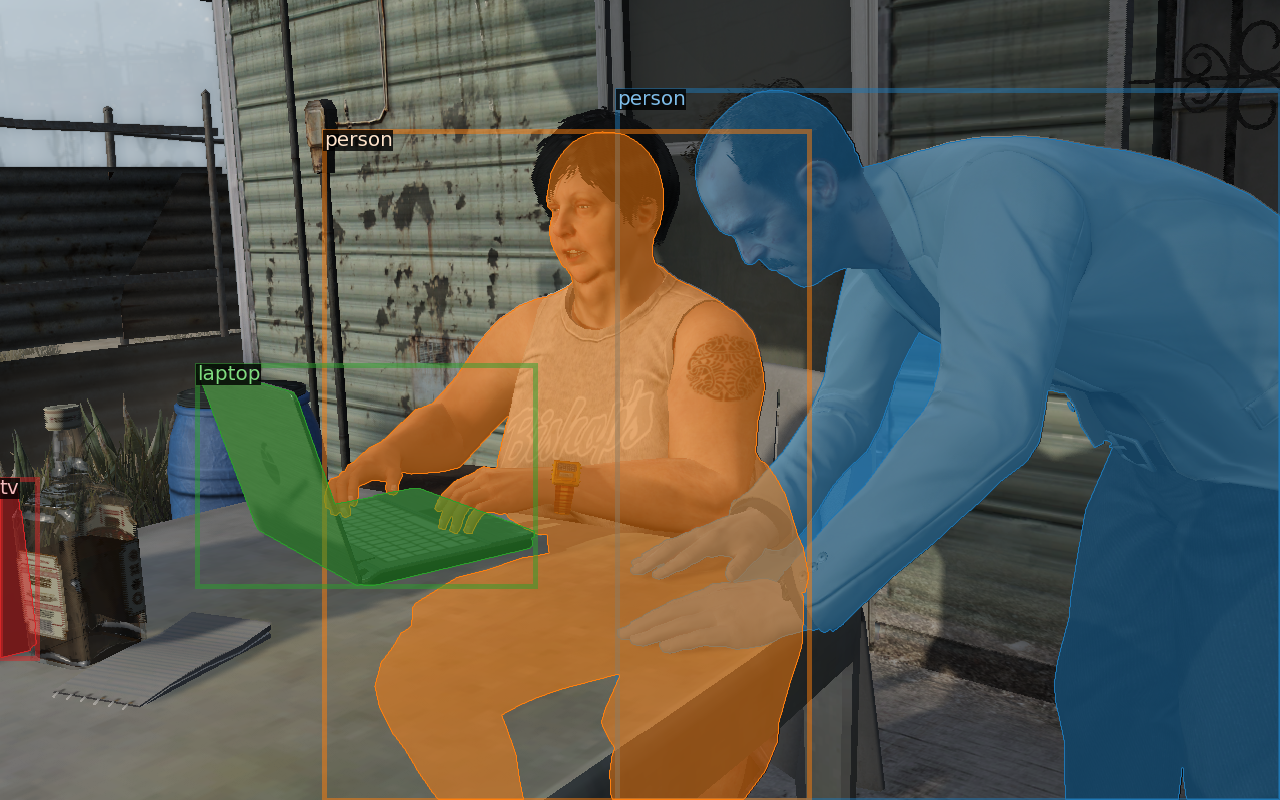
\includegraphics[width=0.31\linewidth]{fig/sailvos_results/21781_gt} &
    %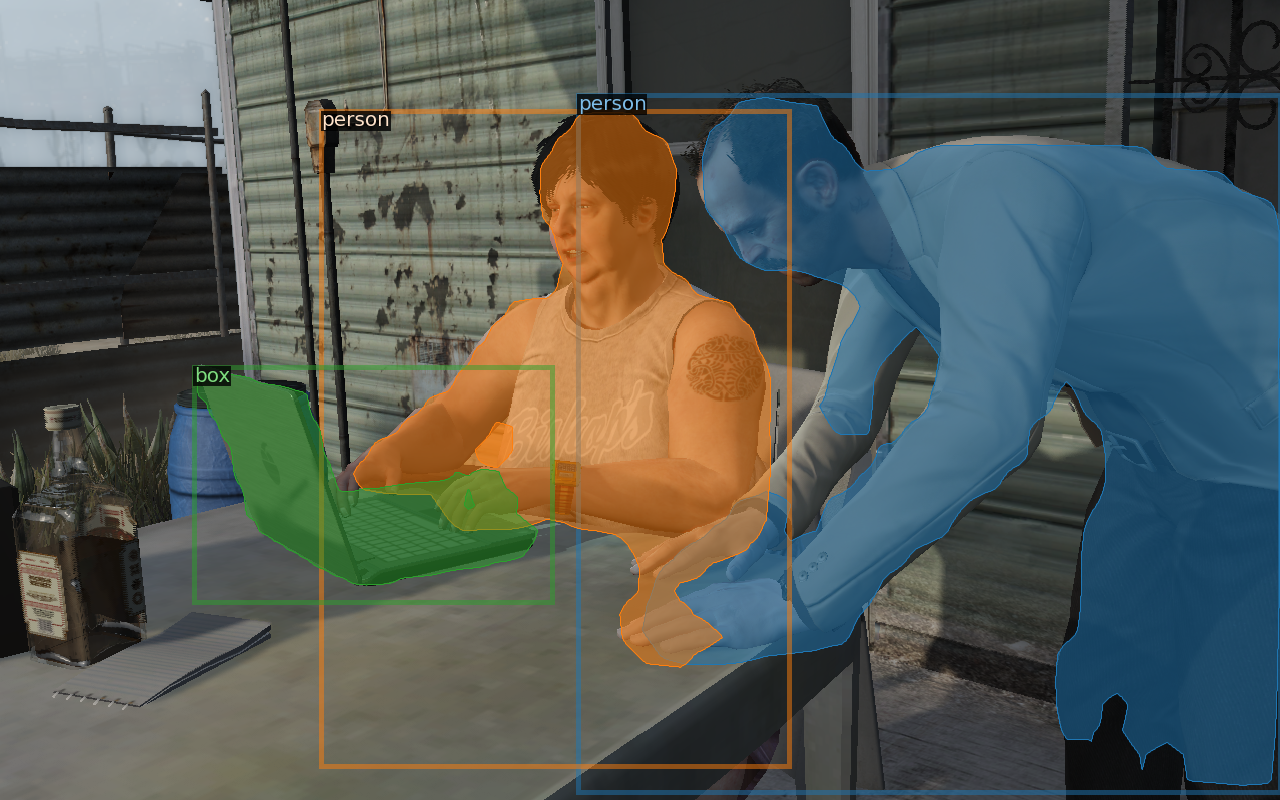
\includegraphics[width=0.31\linewidth]{fig/sailvos_results/21781_base} &
    %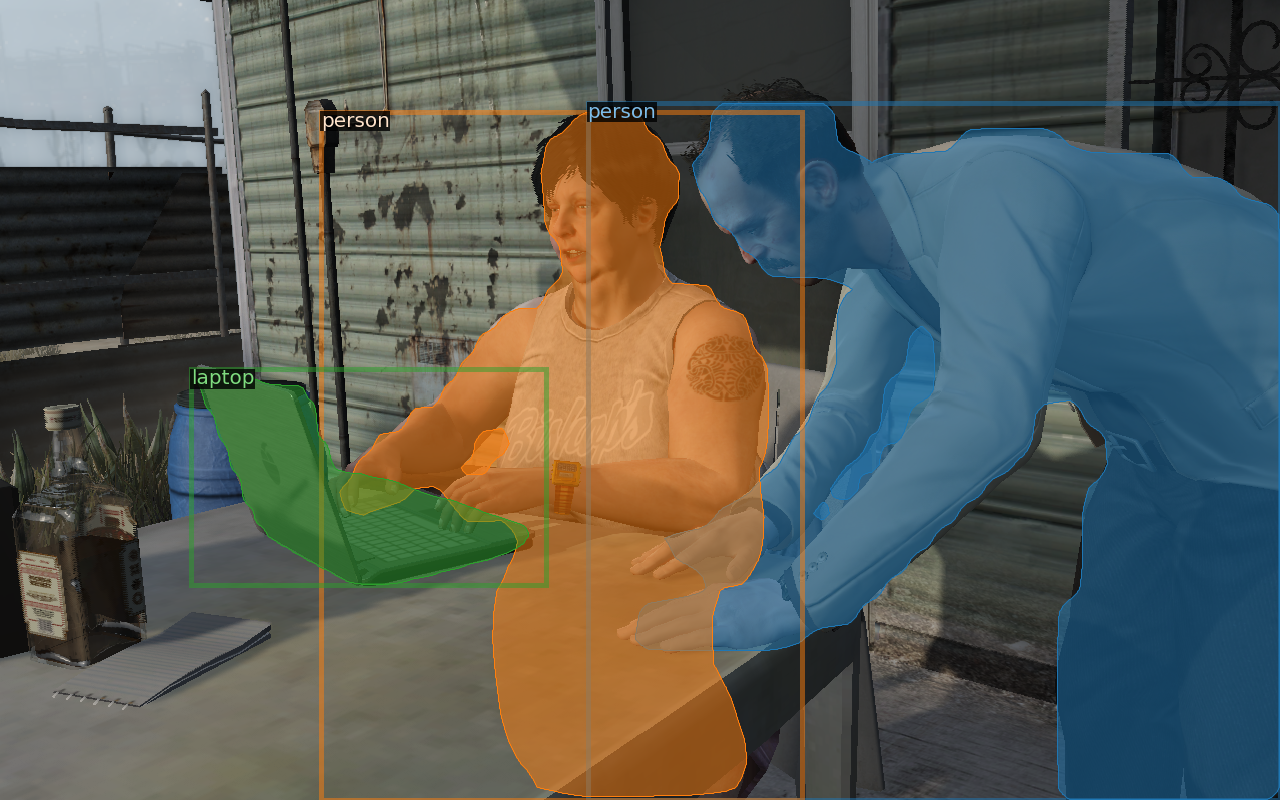
\includegraphics[width=0.31\linewidth]{fig/sailvos_results/21781_ours}\\
    %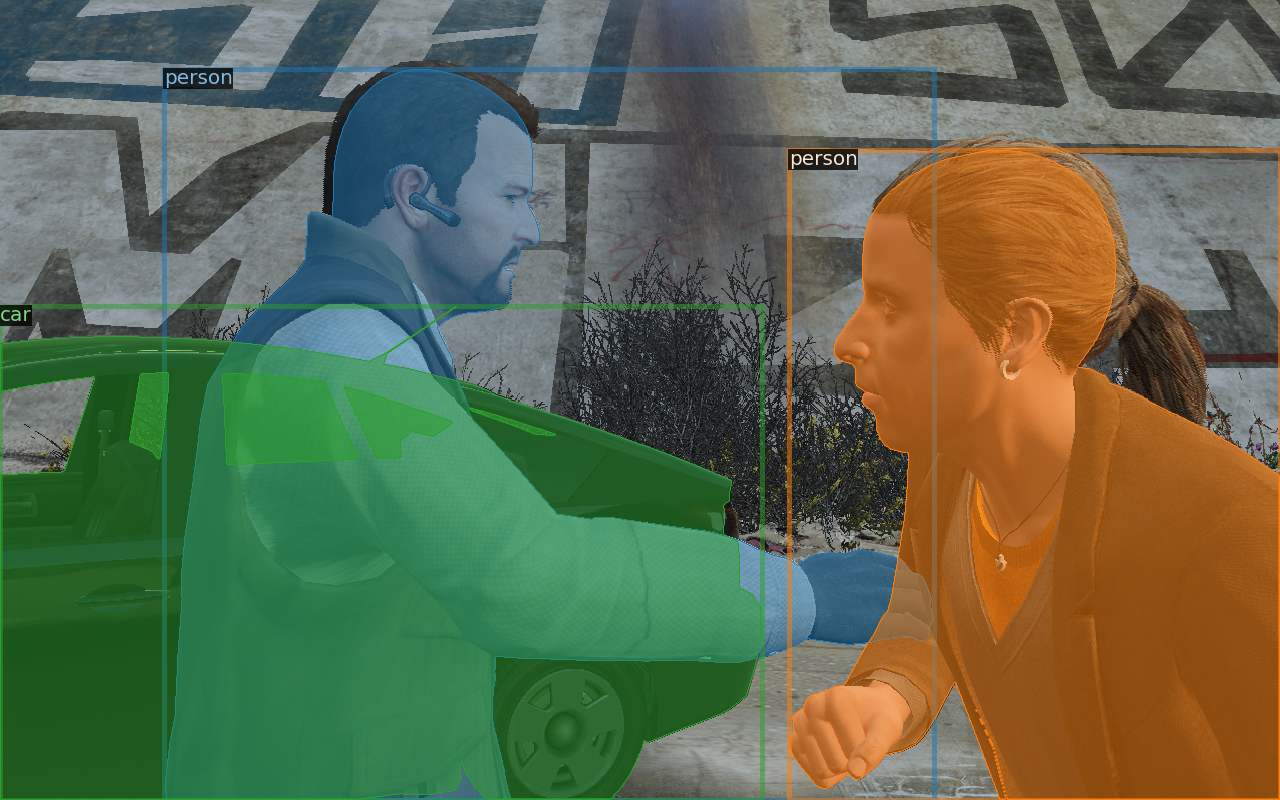
\includegraphics[width=0.31\linewidth]{fig/sailvos_results/11413_gt} & 
    %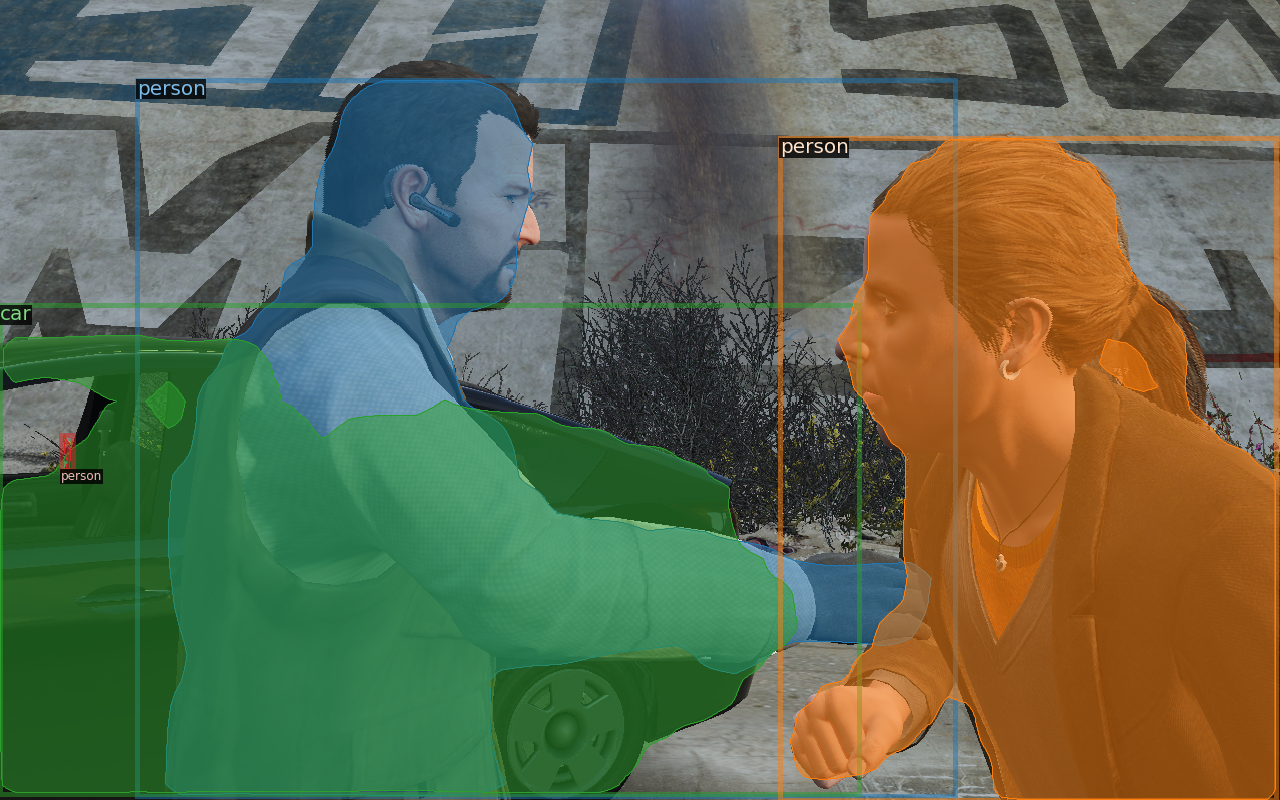
\includegraphics[width=0.31\linewidth]{fig/sailvos_results/11413_base} & 
    %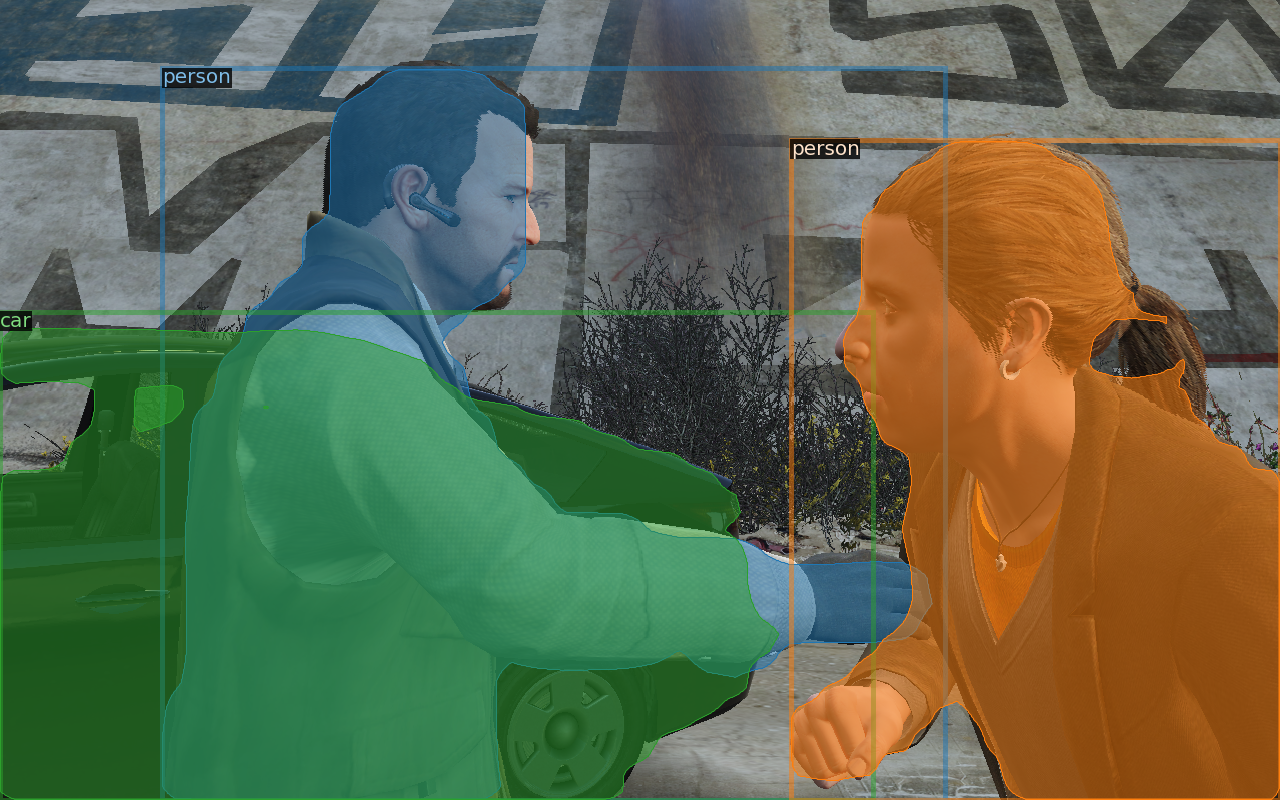
\includegraphics[width=0.31\linewidth]{fig/sailvos_results/11413_ours}\\
    %GT & MaskJoint & Ours
    %\end{tabular}
    
    %\begin{figure*}[t]
    %{
    %\centering
    %\includegraphics[width=0.99\textwidth]{fig/sailvos_results/21781}
    %\includegraphics[width=0.99\textwidth]{fig/sailvos_results/14498}\\
    %}
    %\hspace{2.9cm}Ground-Truth  \hspace{2.8cm} MaskJoint~\cite{hu2019sail}  \hspace{3.2cm} Oursz
    %\caption{Qualitative comparisons with~\cite{hu2019sail} on SAILVOS dataset. 
    %}
    %\label{fig:qual_result}
    %\end{figure*}
    
%!TEX root = ../main.tex
\begin{table*}[t]
\centering
\renewcommand{\arraystretch}{0.95}
\begin{tabular*}{\textwidth}{@{\extracolsep{\fill}}c|ccccccccc}
\specialrule{.15em}{.05em}{.05em}
Row \# & Method &  Occlude & Flow & \# Mask Layers & Cascade & Soft-NMS & Mask Iter. & Box AP & Mask AP\\
\hline\hline
%MaskAmodal~\cite{follmann2019learning} & \xmark & \xmark & 4 & \xmark & \xmark & \xmark & - & 13.0\\ 
%MaskJoint~\cite{hu2019sail} & \xmark & \xmark & 4 & \xmark & \xmark & \xmark & - & 14.1\\
1 & MaskJoint~\cite{hu2019sail} & \xmark&  \xmark & 4 & \xmark & \xmark  & \xmark & - & 14.1\\
2 & Ours & \cmark & \xmark & 4 & \xmark & \xmark  & \xmark & 16.4 & 14.6\\
\hline 
3 & Ours & \cmark & \xmark & 9 &\xmark  & \xmark & \xmark & 16.4  & 15.4\\
4 & Ours & \cmark & \xmark & 10 &\xmark  & \xmark & \xmark &  16.4 & 15.3\\
\hline
5 & Ours & \cmark & \cmark & 9 &\xmark  & \xmark & \xmark &  17.5 & 16.3 \\
\hline 
6 & Ours & \cmark & \cmark & 9 &\cmark  & \xmark & \xmark &  18.6 & 16.7 \\
7 & Ours & \cmark & \cmark & 9 &\cmark  & \cmark & \xmark &   19.6 & 17.3\\
8 & Ours & \cmark & \cmark & 9 &\cmark  & \cmark & \cmark &  \bf 19.6 & \bf 17.6\\
%\cite{hu2019sail} & \xmark & \xmark & - & 13.0 & - & -\\

%\hline
%Ours & \xmark & \xmark &  16.24 & 14.15 & - & - \\
%Ours & \cmark & \cmark &   16.40 & 14.58 & 14.47 & 1.502\\
%\hline
%Ours+6conv. & \xmark & \xmark &  16.26 & 14.90 & - & -\\
%Ours+6conv. & \cmark & \cmark & 16.40  & 15.39 & 14.98 & 2.002\\
%Ours+5conv. & \cmark & \cmark & 16.40  & 15.39 & 14.98 & 2.002\\
%\hline
%Ours+5conv.+flow+soft\_nms & \cmark & \cmark & \bf 17.47 & \bf 16.25 & \bf 15.82 & \bf 2.079\\
\specialrule{.15em}{.05em}{.05em}
\end{tabular*}
\vspace{-0.3cm}
\caption{Ablation study for each of the proposed components on the SAIL-VOS dataset using the class-specific setting.}
\label{tab:abalation}
\vspace{-0.5cm}
\end{table*}



\section{Metrics and Baseline}

To evaluate amodal segmentation, we report the commonly used average precision (AP) averaged over IoU thresholds from $50\%$ to $95\%$. We also report AP with an IoU threshold of 50\%, \ie, $\text{AP}_{50}$. To further study the results, we compute a range of metrics, including $\text{AP}_{\text{50}}^{\text{P}}$ and  $\text{AP}_{\text{50}}^{\text{H}}$. Both report the $\text{AP}_{50}$ using a subset of instances containing (P)artial ($<25\%$) or (H)eavy ($\geq25\%$) occlusions. Similarly, we also report across different instance sizes, $\text{AP}_{\text{50}}^{\text{L}}$, $\text{AP}_{\text{50}}^{\text{M}}$, and $\text{AP}_{\text{50}}^{\text{S}}$ which correspond to pixel area of (L)arge ($\geq 96^2$), (M)edium ($[32^2, 96^2]$), and (S)mall ($\leq 32^2$)  box areas respectively. 

We compare our approach to two recent Mask-RCNN-based amodal segmentation methods, {\it MaskAmodal}~\cite{follmann2019learning}  and {\it MaskJoint}~\cite{hu2019sail}. MaskAmodal directly trains the Mask-RCNN on the task of amodal mask prediction. Differently, MaskJoint learns both amodal and model mask prediction simultaneously by introducing another mask-head into Mask-RCNN.


\section{SAIL-VOS Dataset}
The SAIL-VOS dataset consists of $160$ training and $41$ validation video sequences with $800 \times 1,280$ resolution images annotated with amodal/modal boxes and segmentation masks. The dataset has $111654$ images in total; 26873 images are used for testing, and 84781 images are used for training. There are $1896295$ instances labeled in total. 
Following Hu~\etal~\cite{hu2019sail}, objects with occlusion rate larger than $75\%$ are excluded from training and testing. We consider two common experimental settings: the class-specific setting which focuses on a 24 class subset within the dataset, and a class-agnostic setting which disregards the class-labels and views all objects to be of a single class. In the Amodal-net experiements, both settings are studied. Only the class-specific setting is studied in the experiements with reprojection.





\section{Sanity Check Experiments}
Before adding reprojection to the network, I conducted some sanity check experiments to evaluate the effect of reprojection. 

My first experiment is to evaluate the gain on AP from doing reprojection. Here are the quantative results in \tabref{tab:sanity}. The first three lines are from Amodal-net. The last four lines are the evaluation of using groundtruth masks from $t-1$ or $t-2$ as prediction, with or without reprojection. As one would expect, the accuracy of the lines that is using reprojection is higher, confirming our presumption that reprojection should allow us to use 3D and temporal information better. But obviously these lines are using modified versions of groundtruth masks, and hence are not comparable to the first three lines. The final goal of this project would be to incorporate this reprojected information into the training pipeline to improve the numbers in the third line.

My second experiment is training a small network ($1 \times 1$ convolution) on the groundtruth reprojected masks from previous frames. I use one-hot encoding, so each training input has shape $(25*n) \times h \times w$, where $25$ is the number of categories (plus 1 for background) and $n$ is the number of previous masks we passed in the network. The first version I trained has the masks from frames $t,t-1,t-2,t-3$. As one would expect, the model learned to take the groundtruth mask from $t$ directly as output, and achieved perfect accuracy. \ref{fig:w4} shows the weight that the model learned. The x-axis is the the input channels and the y-axis is the output channels. The model correctly learns to use the main diagonal primarily, correponding to using the groundtruth mask from the frame $t$. In the next version, I only passed in groundtruth masks from $t-1,t-2,t-3$ as input. As shown in \ref{fig:w3}, the weights are largest in the three diagonals as one would expect. Out of the three diagonals, the main diagonal is the largest. It is consistent with our expectation that the the most recent mask ($t-1$) is the most valuable. But it is good to see that the model is also using mask from $t-2$ and $t-3$ frames to some extent. This further confirms our presumption that the reprojected masks from previous frames would help with the performance of the model. I also explored how some hyper-parameters impact the training process. Finally, I launched a training with a $3\times 3$ convolutional network with the same parameters. It did not perform too much better than the $1\times 1$ one. 

\ref{tab:sanity} shows the quantitative results of these sanity check experiments. The convolutional networks performs slightly better than directly using the groundtruth $t-1$ mask, which makes sense since that is the most recent mask. The plots \ref{fig:plot1} of the predicted mask also match this.

\begin{figure}
\centering
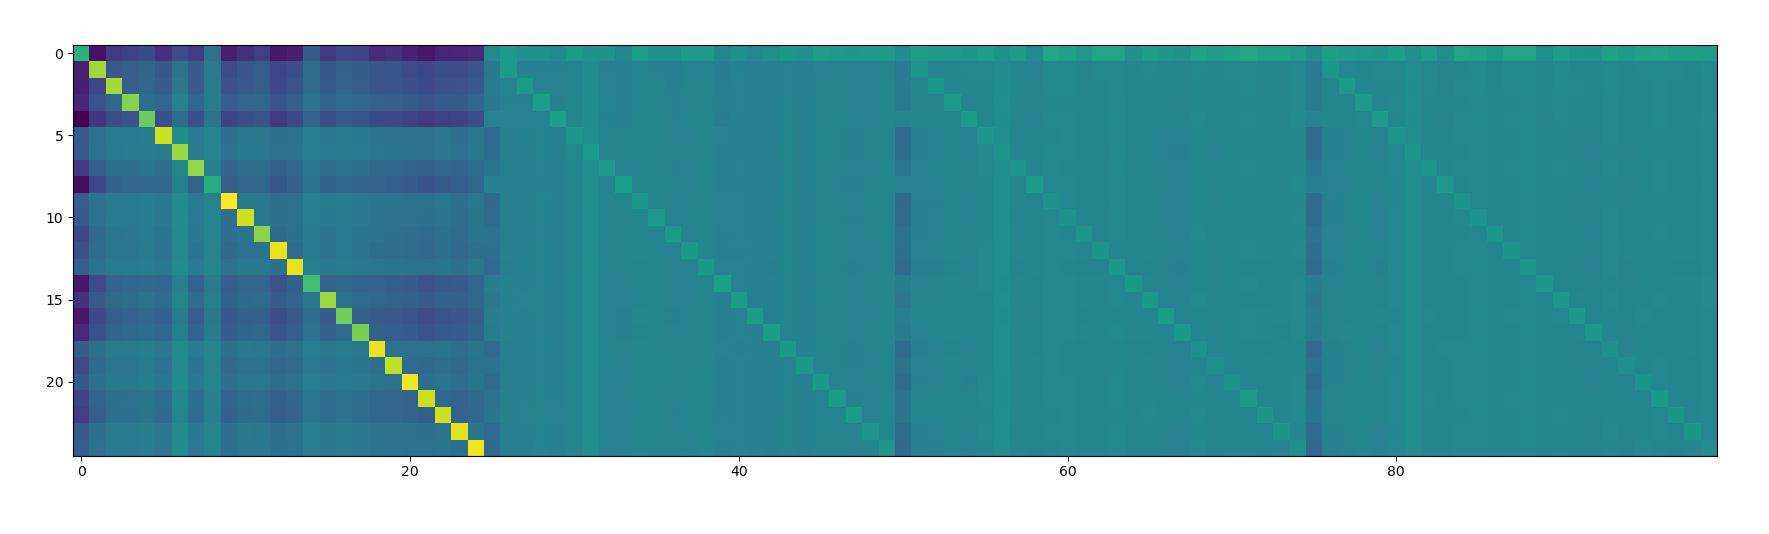
\includegraphics[scale=0.22]{fig/weights_4.png}
\caption{Weight that the model learned. Input is gt masks from t,t-1,t-2,t-3}
\label{fig:w4}
\end{figure}
\begin{figure}
\centering
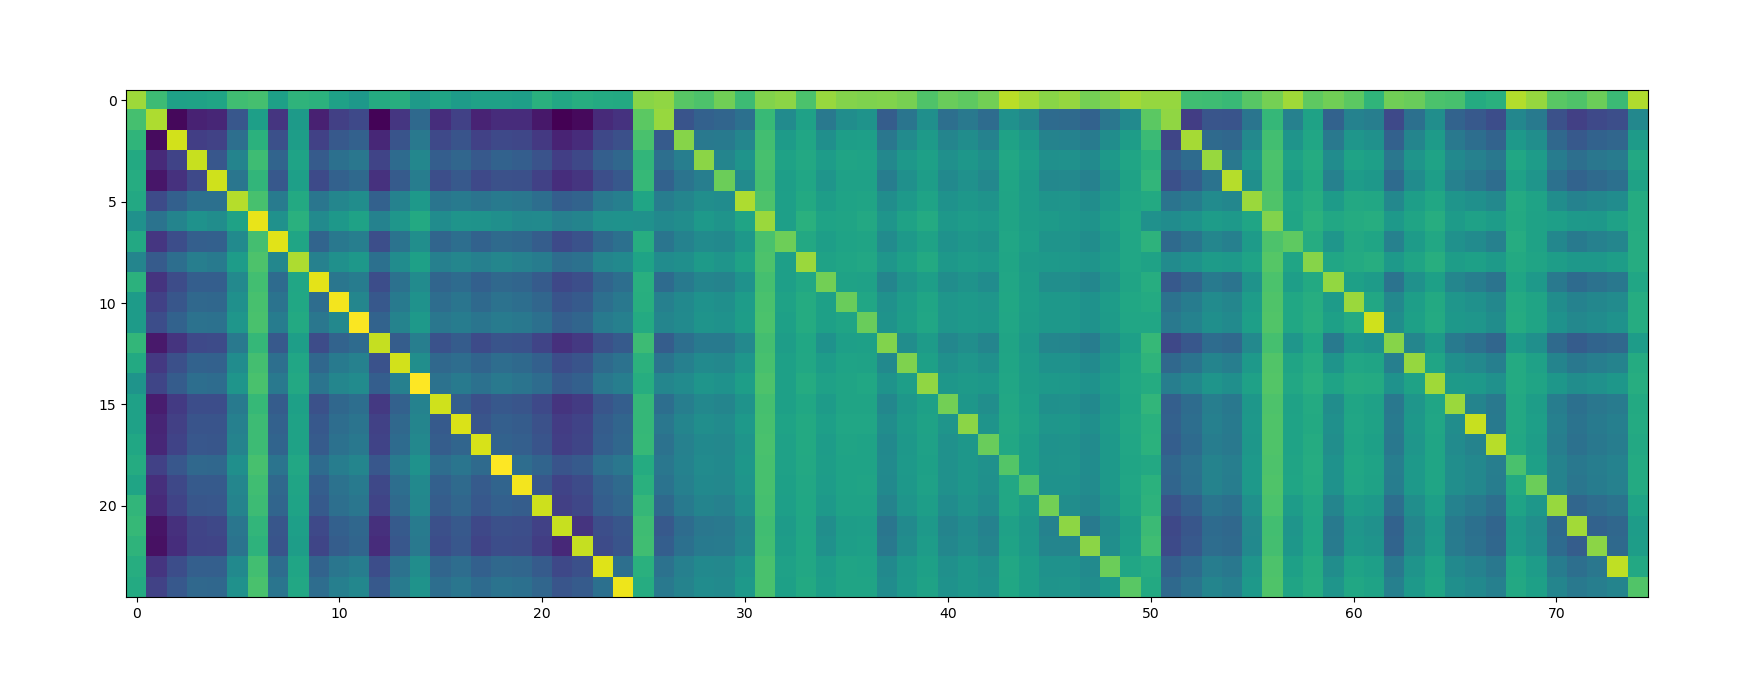
\includegraphics[scale=0.22]{fig/weights_3.png}
\caption{Weight that the model learned. Input is gt masks from t,t-1,t-2,t-3}
\label{fig:w3}
\end{figure}

\begin{figure}
\centering

\includegraphics[scale=0.23]{fig/pred.png}
\caption{gt mask, t-1 mask, t-2 mask,t-3 mask and predicted mask. The prediction is from 1x1 conv network that is trained without gt}
\label{fig:plot1}
\end{figure}

%!TEX root = ../main.tex
\begin{table*}[t]
%\small
\centering
\setlength{\tabcolsep}{4pt}
\renewcommand{\arraystretch}{0.95}
\begin{tabular*}{\textwidth}{@{\extracolsep{\fill}}c|cccccccc}
\specialrule{.15em}{.05em}{.05em}
 %@{\extracolsep{\fill}}
& \multicolumn{7}{c}{\bf SAIL-VOS class-specific} &  \\
Method & AP &  $\text{AP}_{\text{50}}$ & $\text{AP}_{\text{50}}^{\text{P}}$ & $\text{AP}_{\text{50}}^{\text{H}}$ & $\text{AP}_{\text{50}}^{\text{L}}$ & $\text{AP}_{\text{50}}^{\text{M}}$ & $\text{AP}_{\text{50}}^{\text{S}}$ 

\\
\hline\hline
MaskAmodal~ & 
13.0 & 23.0 & 24.3 & 16.7 & 36.6 & 21.5 & 6.1 & \\% Class-specific

%40.4 & 26.6\\

MaskJoint~\cite{hu2019sail} &
14.1 & 24.8 & 24.3 & 18.9 & 37.8 & 21.5 & 5.7 & \\  % Class-specific

Amodal-net & 
\bf 17.6 & \bf 28.3 &  \bf 28.9 & \bf 20.1 &  \bf 47.1 & \bf 24.8 & \bf 10.6& \\% Class-Agnostic

\hline
Gt t-1 frame w/o reprojection & 
 - &  61.7 &   53.6 &  50.5 &   - & - & -& \\ % Class-Agnostic


Gt t-1 frame w reprojection & 
 - &  69.3 &   61.8 &  58.0 &   - &  - &  -& \\

Gt t-2 frame w/o reprojection & 
 - &  50.4 &  43.3 & 37.7 &  - &  - &  -& \\

Gt t-2 frame w reprojection & 
 - & \bf 64.5 &  \bf 56.7 & \bf 51.8 &  - &  - &  -& \\


Gt t-2 frame w/o reprojection & 
 - &  64.5 &   56.7 &  51.8 &  - &  - &  -& \\

1x1 Conv w/ gt t,t-1,t-2, t-3 frames w reprojection &
- &  99.9 &   99.9 &  99.9 &  - &  - &  -& \\


\hline
1x1 Conv w/ gt t-1,t-2, t-3 frames w reprojection &
- &  \bf 69.4 &  \bf 61.9 &  58.2 &  - &  - &  -& \\

3x3 Conv w/ gt t-1,t-2, t-3 frames w reprojection &
- &  69.4 &   61.8 & \bf 58.4 &  - &  - &  -& \\
\specialrule{.15em}{.05em}{.05em}
\end{tabular*}
\vspace{-0.3cm}
\caption{Quantitative amodal segmentation results for sanity check of reprojection
%\ray{Class-agnostic heavy needs some tunining?}
}
\vspace{-0.45cm}
\label{tab:sanity}
\end{table*}



\section{Experiment with Reprojection}
In the main experiment, I implemented the reprojection in the feature space. As shown in \ref{fig:pipeline}, the main part I added is annotated in red. In the dataloader, I added the depth map of the images and the camera matrices in addition to the images theselves. Then in the network, I added a layer that reproject the feature from one frame to another as in \ref{chp:approach}. In the implementation, I had to change the reprojection code to accomodate reprojection in the feature space instead of for the image directly. Since it is of a lower resolution, I needed to downsample the depth map. I tried a few difference modes of resizing to get the minimum amount of the aliasing effect. In the end I found that just using the nearest performs the best. The results of this experiment are discussed in \ref{chp:res}

